\documentclass[notheorems,serif]{beamer}

%选用主题
\usetheme{Madrid}

\usepackage[no-math, cm-default]{fontspec}
\usepackage{xltxtra}
\usepackage{xunicode}   
\usepackage{xcolor}
%\usepackage{unicode-math} % 使用 unicode-math 设置数学字体
\usepackage{amsmath, amssymb}
\usepackage{xeCJK}
\usepackage{multimedia}
\usepackage{listings}
\usepackage{caption}
\usepackage{multirow}
\usepackage{color, subcaption}
\usepackage{makecell}
\usepackage{algorithm}
\usepackage{algpseudocode}

%将系统字体名映射为逻辑字体名称,主要是为了维护的方便  
\newcommand\fnhei{Adobe 黑体 Std}  
\newcommand\fnsong{Adobe 宋体 Std}  
\newcommand\fnkai{Adobe 楷体 Std}  
\newcommand\fnmono{DejaVu Sans Mono}  
\newcommand\fnroman{Times New Roman}  

% 定理类环境的定义
\newtheorem{definition}{定义}[section]
\newtheorem{property}{性质}[section]
\newtheorem{lemma}{引理}[section]
\newtheorem{theorem}{定理}[section]
\newtheorem{corollary}{推论}[section]
\newtheorem{example}{算例}
\newtheorem{remark}{注}
\newtheorem{assumption}{假设}
\newtheorem{continue}{续}

\newcommand{\highlightit}{\textcolor[rgb]{1.00,0.00,0.00}}


%---SHORTCUTS--------------------------------------------------------------------------------------
\newcommand\xor{\mathbin{\char`\^}}
\DeclareMathOperator{\res}{Res}
\DeclareMathOperator{\sgn}{sgn}
\DeclareMathOperator{\supp}{supp}
\DeclareMathOperator{\as}{as}
\newcommand{\slant}[1]{\slshape #1\normalfont}
\newcommand{\dd}[2]{\frac{d#1}{d#2}} 
\newcommand{\ddx}{\frac{d}{dx}}
\newcommand{\ddt}{\frac{d}{dt}}
\newcommand{\dds}{\frac{d}{ds}}
\newcommand{\pd}[1]{\ds\frac{\partial}{\partial #1 }}
\newcommand{\pdd}[2]{\ds\frac{\partial #1}{\partial #2 }}
\newcommand{\mdd}[3]{\ds\frac{\partial^{#3} #1}{\partial #2^{#3} }}
\newcommand{\x}{\ _\Box}
\newcommand{\ds}{\displaystyle}
\newcommand{\Bold}{\noindent \bfseries}
\newcommand{\Norm}{\normalfont}
\newcommand{\exl}[1]{\textcolor{NavyBlue}{\Bold Exercise #1 \Norm}}
\newcommand{\ex}{\textcolor{NavyBlue}{\Bold Problem: \Norm}}
\newcommand{\sol}{\textcolor{Mulberry}{\Bold Solution: \Norm}}
\newcommand{\pf}{\textcolor{Mulberry}{\Bold Proof: \Norm}}
\newcommand{\Title}[1]{\LARGE\Bold \textcolor{Sepia}{#1}\Norm\normalsize \vspace{10pt} \newline}
\newcommand{\prop}{\Bold \textcolor{YellowOrange}{ Proposition:} \Norm}
\newcommand{\propl}[1]{\Bold \textcolor{YellowOrange}{ Proposition #1:} \Norm}
\newcommand{\rk}{\Bold \textcolor{YellowOrange}{ Remark:} \Norm}
\newcommand{\rmk}[1]{\Bold\textcolor{YellowOrange}{#1} \Norm}
\newcommand{\thm}[1]{\Bold \textcolor{YellowOrange}{ Theorem #1} \Norm}
\newcommand{\ind}{\indent\indent}

\newcommand{\red}{\color{red}}
\newcommand{\blue}{\color{blue}}

\newcommand{\mycomment}[1]{} % 默认不显示注释








% 定义粗体英文字母
\newcommand{\bsa}{\boldsymbol{a}}
\newcommand{\bsb}{\boldsymbol{b}}
\newcommand{\bsc}{\boldsymbol{c}}
\newcommand{\bsd}{\boldsymbol{d}}
\newcommand{\bse}{\boldsymbol{e}}
\newcommand{\bssf}{\boldsymbol{f}}
\newcommand{\bsg}{\boldsymbol{g}}
\newcommand{\bsh}{\boldsymbol{h}}
\newcommand{\bsi}{\boldsymbol{i}}
\newcommand{\bsj}{\boldsymbol{j}}
\newcommand{\bsk}{\boldsymbol{k}}
\newcommand{\bsl}{\boldsymbol{l}}
\newcommand{\bssm}{\boldsymbol{m}}
\newcommand{\bsn}{\boldsymbol{n}}
\newcommand{\bso}{\boldsymbol{o}}
\newcommand{\bsp}{\boldsymbol{p}}
\newcommand{\bsq}{\boldsymbol{q}}
\newcommand{\bsr}{\boldsymbol{r}}
\newcommand{\bss}{\boldsymbol{s}}
\newcommand{\bst}{\boldsymbol{t}}
\newcommand{\bsu}{\boldsymbol{u}}
\newcommand{\bsv}{\boldsymbol{v}}
\newcommand{\bsw}{\boldsymbol{w}}
\newcommand{\bsx}{\boldsymbol{x}}
\newcommand{\bsy}{\boldsymbol{y}}
\newcommand{\bsz}{\boldsymbol{z}}

\newcommand{\bsA}{\boldsymbol{A}}
\newcommand{\bsB}{\boldsymbol{B}}
\newcommand{\bsC}{\boldsymbol{C}}
\newcommand{\bsD}{\boldsymbol{D}}
\newcommand{\bsE}{\boldsymbol{E}}
\newcommand{\bsF}{\boldsymbol{F}}
\newcommand{\bsG}{\boldsymbol{G}}
\newcommand{\bsH}{\boldsymbol{H}}
\newcommand{\bsI}{\boldsymbol{I}}
\newcommand{\bsJ}{\boldsymbol{J}}
\newcommand{\bsK}{\boldsymbol{K}}
\newcommand{\bsL}{\boldsymbol{L}}
\newcommand{\bsM}{\boldsymbol{M}}
\newcommand{\bsN}{\boldsymbol{N}}
\newcommand{\bsO}{\boldsymbol{O}}
\newcommand{\bsP}{\boldsymbol{P}}
\newcommand{\bsQ}{\boldsymbol{Q}}
\newcommand{\bsR}{\boldsymbol{R}}
\newcommand{\bsS}{\boldsymbol{S}}
\newcommand{\bsT}{\boldsymbol{T}}
\newcommand{\bsU}{\boldsymbol{U}}
\newcommand{\bsV}{\boldsymbol{V}}
\newcommand{\bsW}{\boldsymbol{W}}
\newcommand{\bsX}{\boldsymbol{X}}
\newcommand{\bsY}{\boldsymbol{Y}}
\newcommand{\bsZ}{\boldsymbol{Z}}

% 定义粗体希腊字母
\newcommand{\balpha}{\boldsymbol{\alpha}}
\newcommand{\bbeta}{\boldsymbol{\beta}}
\newcommand{\bgamma}{\boldsymbol{\gamma}}
\newcommand{\bdelta}{\boldsymbol{\delta}}
\newcommand{\bzeta}{\boldsymbol{\zeta}}
\newcommand{\btheta}{\boldsymbol{\theta}}
\newcommand{\blambda}{\boldsymbol{\lambda}}
\newcommand{\bmu}{\boldsymbol{\mu}}
\newcommand{\bnu}{\boldsymbol{\nu}}
\newcommand{\bxi}{\boldsymbol{\xi}}
\newcommand{\brho}{\boldsymbol{\rho}}
\newcommand{\bsigma}{\boldsymbol{\sigma}}
\newcommand{\btau}{\boldsymbol{\tau}}
\newcommand{\bphi}{\boldsymbol{\phi}}
\newcommand{\bomega}{\boldsymbol{\omega}}
\newcommand{\bpi}{\boldsymbol{\pi}}
\newcommand{\bPi}{\boldsymbol{\Pi}}
\newcommand{\bSigma}{\boldsymbol{\Sigma}}
\newcommand{\bOmega}{\boldsymbol{\Omega}}


\newcommand{\dof}{\operatorname{dof}}
\newcommand{\curl}{\operatorname{curl}}
\newcommand{\diver}{\mathrm{div}}
\newcommand{\bcurl}{\mathbf{curl}}
\newcommand{\diag}{\mathrm{diag}}
\newcommand{\sign}{\mathrm{sign}}
\newcommand{\grad}{\mathbf{grad}}
\newcommand{\sym}{\mathrm{sym}}
\newcommand{\rot}{\operatorname{rot}}
\newcommand{\brot}{\operatorname{\mathbf{rot}}}

%---SCRIPT-----------------------------------------------------------------------------------------
\newcommand{\cA}{\mathcal{A}}
\newcommand{\cB}{\mathcal{B}}
\newcommand{\cC}{\mathcal{C}}
\newcommand{\cD}{\mathcal{D}}
\newcommand{\cE}{\mathcal{E}}
\newcommand{\ce}{\mathcal{e}}
\newcommand{\cF}{\mathcal{F}}
\newcommand{\cG}{\mathcal{G}}
\newcommand{\cg}{\mathcal{g}}
\newcommand{\cH}{\mathcal{H}}
\newcommand{\cI}{\mathcal{I}}
\newcommand{\cJ}{\mathcal{J}}
\newcommand{\cK}{\mathcal{K}}
\newcommand{\cL}{\mathcal{L}}
\newcommand{\cM}{\mathcal{M}}
\newcommand{\cN}{\mathcal{N}}
\newcommand{\cO}{\mathcal{O}}
\newcommand{\cP}{\mathcal{P}}
\newcommand{\cQ}{\mathcal{Q}}
\newcommand{\cR}{\mathcal{R}}
\newcommand{\cS}{\mathcal{S}}
\newcommand{\cT}{\mathcal{T}}
\newcommand{\cU}{\mathcal{U}}
\newcommand{\cV}{\mathcal{V}}
\newcommand{\cW}{\mathcal{W}}
\newcommand{\cX}{\mathcal{X}}
\newcommand{\cY}{\mathcal{Y}}
\newcommand{\cZ}{\mathcal{Z}}
\newcommand{\cz}{\mathcal{z}}
%---BLACKBOARD-------------------------------------------------------------------------------------
\newcommand{\mA}{\mathbb A}
\newcommand{\mB}{\mathbb B}
\newcommand{\mC}{\mathbb C}
\newcommand{\mD}{\mathbb D}
\newcommand{\mE}{\mathbb E}
\newcommand{\mF}{\mathbb F}
\newcommand{\mG}{\mathbb G}
\newcommand{\mg}{\mathbb g}
\newcommand{\mH}{\mathbb H}
\newcommand{\mI}{\mathbb I}
\newcommand{\mJ}{\mathbb J}
\newcommand{\mK}{\mathbb K}
\newcommand{\mL}{\mathbb L}
\newcommand{\mM}{\mathbb M}
\newcommand{\mN}{\mathbb N}
\newcommand{\mO}{\mathbb O}
\newcommand{\mP}{\mathbb P}
\newcommand{\mQ}{\mathbb Q}
\newcommand{\mR}{\mathbb R}
\newcommand{\mS}{\mathbb S}
\newcommand{\mT}{\mathbb T}
\newcommand{\mU}{\mathbb U}
\newcommand{\mV}{\mathbb V}
\newcommand{\mW}{\mathbb W}
\newcommand{\mX}{\mathbb X}
\newcommand{\mY}{\mathbb Y}
\newcommand{\mZ}{\mathbb Z}
\newcommand{\mz}{\mathbb z}

\newcommand{\bH}{\mathbf{H}}
\newcommand{\bu}{\mathbf{u}}
\newcommand{\bfx}{\mathbf{x}}
\newcommand{\ddiv}{\operatorname{div}}
\newcommand{\bfV}{\mathbf{V}}
\newcommand{\bv}{\mathbf{v}}

\newcommand{\dist}{\operatorname{dist}}

\newcommand{\bzero}{\mathbf{0}}
\newcommand{\bka}{\mathbf{\kappa}}

\newcommand{\rd}{\mathrm{d}}


\begin{document}

\title{博士毕业答辩:新型虚单元方法的理论及应用研究}
\author{答辩人:陈春雨\\
\vspace{5pt}
导师:{\CJKfontspec{SimSun}魏华祎} 教授}

\institute[XTU]{
    \vspace{5pt}
\vspace{5pt}
 
湘潭大学\\
数学与计算科学学院\\
}

\date
{
    \today
}

%\pgfdeclareimage[height=1cm]{institution-logo}{../figures/xtu.pdf}
%\logo{\pgfuseimage{institution-logo}}
\frame[plain]{\titlepage}
\AtBeginSection[]{
  \frame<beamer>{ 
    \frametitle{Outline}   
    \tableofcontents[currentsection] 
  }
}

\section{虚单元方法}
\begin{frame}
  \frametitle{虚单元方法}
虚单元方法是一种新型偏微分方程数值求解方法,由 
F.Brezzi 等人于 2013 年提出([L. Beirão da Veiga et al., 2013])。

\begin{figure}[htbp]
\centering
\begin{subfigure}[t]{0.49\linewidth}
    \centering
    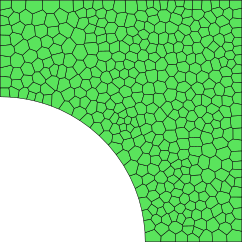
\includegraphics[width=1.6in]{../figures/voronoi_quad_circle.pdf}
\end{subfigure}%
\begin{subfigure}[t]{0.49\linewidth}
    \centering
    \includegraphics[width=2.5in]{../figures/bird.png}
\end{subfigure}%
\caption{虚单元方法适用的网格。左:使用 FEALPy 生成的多边形网格;右:使用
Vorocrust 生成的多面体网格。}
\label{fig:all}
\end{figure}

\end{frame}

\begin{frame}\frametitle{Poisson 方程}
\begin{minipage}[b]{0.6\linewidth}
考虑 $\Omega$ 上的 Poisson 方程问题:
$$
\left\{
\begin{aligned}
-\Delta u &= f \quad \text{in} \quad \Omega, \\
u &= 0 \quad \text{on} \quad \partial \Omega,
\end{aligned}
\right.
$$
其中 $f \in L^2(\Omega)$.
对应的变分问题为:找到 $u \in H^1_0(\Omega)$ 使得
$$
a(u, v) = (f, v) \quad \forall v \in H^1_0(\Omega),
$$
其中
$$
a(u, v) = \int_{\Omega} \nabla u \cdot \nabla v \, \mathrm{d} x.
$$
\end{minipage}
\hfill
\begin{minipage}[b]{0.38\linewidth}
    \centering
    \begin{figure}[htpb]
        \centering
        
\includegraphics[width=0.65\textwidth]{../figures/domain_quad.pdf}
        \caption{计算区域 $\Omega$.}
    \end{figure}
\end{minipage}

\end{frame}

%\begin{frame}
%    \frametitle{Poisson 方程的线性有限元方法}
%\begin{itemize}
%\item 将 $\Omega$ 划分为三角形网格 $\mathcal{T}_h$.
%\end{itemize}
%\vspace{10pt}
%\begin{figure}[htpb]
%    \centering
%    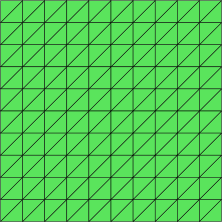
\includegraphics[width=0.4\textwidth]{../figures/struct_triangle_mesh.pdf}
%    \caption{三角形网格 $\mathcal{T}_h$.}
%\end{figure}
%\end{frame}
%
%\begin{frame}
%\begin{itemize}
%\item 定义有限元 $(V_k^K, K, \mathcal{N})$,其中 $V_k^K := \mathbb{P}_1(K)$.
%    自由度 $\mathcal{N}$ 是函数在顶点处的值:
%    $$
%    \mathcal{N}_i(v) = v(x_i)
%    $$
%\end{itemize}
%\begin{figure}[htpb]
%    \centering
%    \includegraphics[width=1.0\textwidth]{../figures/fembasis.pdf}
%    \caption{线性元局部基函数.}
%\end{figure}
%\end{frame}
%
%\begin{frame}
%\begin{itemize}
%\item 构造全局有限元空间 $V_k$:
%    $$
%    V_k = \{v_h \in H^1(\Omega): v_h|_K \in V_k^K, \forall K \in
%    \mathcal{T}_h\}.
%    $$
%\end{itemize}
%\begin{figure}[htpb]
%    \centering
%    \includegraphics[width=0.6\textwidth]{../figures/femfunction_global.png}
%    \caption{线性元全局基函数.}
%\end{figure}
%\end{frame}
%
%\begin{frame}
%\begin{itemize}
%\item 
%    求解有限元问题 :找到 $u_h \in V_k$ 使得
%    $$
%    a_h(u_h, v_h) = (f, v_h) \quad \forall v_h \in V_k,
%    $$
%    其中
%    $$
%    a_h(u_h, v_h) = \sum_{K \in \mathcal{T}_h} \int_K \nabla u_h \cdot \nabla v_h \,
%    \mathrm{d} x
%    $$
%\end{itemize}
%\end{frame}

\begin{frame}
    \frametitle{Poisson 方程的虚单元方法}
\begin{itemize}
    \item 将 $\Omega$ 划分为多边形网格 $\mathcal{T}_h$.
\end{itemize}
\begin{figure}[htpb]
    \centering
    \includegraphics[width=0.6\textwidth]{../figures/convex.pdf}
    \caption{多边形网格 $\mathcal{T}_h$.}
\end{figure}
\end{frame}

\begin{frame}
\uncover<1->{
    \begin{itemize}
        \item 
            定义局部虚单元 $(V_k^K, K, \mathcal{N})$,其中
            $$
            V_k^K := \{v \in H^1(K): v|_{\partial K} \in \mathbb{P}_1(\partial K),
            \Delta v = 0\}.
            $$ 
            自由度 $\mathcal{N}$ 同样是函数在顶点处的值.
    \end{itemize}
    \begin{figure}[htpb]
        \centering
        \includegraphics[width=0.9\textwidth]{../figures/vemlambda.png}
        \caption{虚单元局部基函数.}
    \end{figure}
}
\uncover<2->{
    \vspace{-5pt}
\centering{
\highlightit{虚单元基函数难以直接计算,但是其到 $\mathbb{P}_1(K)$ 的 
$H^1$ 投影 $\Pi_h^K$ 是已知的.}
}}
\end{frame}

\begin{frame}
    \begin{itemize}
        \item 构造全局虚单元空间
            $$
            V_k = \{v_h \in H^1(\Omega): v_h|_K \in V_k^K, \forall K \in
            \mathcal{T}_h\}.
            $$
    \end{itemize}
    \begin{figure}[htpb]
        \centering
        \includegraphics[width=0.6\textwidth]{../figures/vemfunction_global.png}
        \caption{虚单元全局基函数.}
    \end{figure}
\end{frame}

\begin{frame}
\frametitle{虚单元方法求解步骤}

\begin{itemize}
\item 求解虚单元问题:寻找 $u_h \in V_k$ 使得
$$
a_h(u_h, v_h) = (f, \Pi_h v_h) \quad \forall v_h \in V_k,
$$
其中离散双线性形式 $a_h$ 定义为:
$$
a_h(u_h, v_h) = \sum_{K \in \mathcal{T}_h} a_h^K(u_h, v_h) 
$$
局部双线性形式 $a_h^K$ 定义为:
$$
\begin{aligned}
a_h^K(u_h, v_h) = & \int_K \nabla \Pi_h^K u_h \cdot \nabla \Pi_h^K v_h \, \mathrm{d}x
\uncover<2->{
\highlightit{+ S_h^K(u_h - \Pi_h^K u_h, v_h - \Pi_h^K v_h)}.
}
\end{aligned}
$$
\uncover<3->{
其中 $S_h^K$ 是稳定项,需要满足:
$$
C_* |v|_{1} \leq S_h^K(v, v) \leq C^* |v|_{1}\quad
\forall v \in \ker{\Pi_h^K} \cap V_k^K.
$$
}
\end{itemize}
\end{frame}

\begin{frame}
  \frametitle{虚单元方法优势:网格的灵活性}
\begin{itemize}
    \item 虚单元方法可以在任意多边形网格上进行计算,即使是带有悬点的网格。
\end{itemize}
\begin{figure}[htbp]
\centering
\begin{subfigure}[t]{0.32\linewidth}
    \centering
    \includegraphics[width=1.0in]{../figures/convex0.pdf}
\end{subfigure}%
\begin{subfigure}[t]{0.32\linewidth}
    \centering
    \includegraphics[width=1.0in]{../figures/nonconvex0.pdf}
\end{subfigure}%
\begin{subfigure}[t]{0.32\linewidth}
    \centering
    \includegraphics[width=1.0in]{../figures/four.jpg}
\end{subfigure}%
\caption{基于 FEALPy 生成的虚单元方法适用的网格。
左:凸网格;中:非凸网格;右:带有悬点的网格。}
\label{fig:all}
\end{figure}
\end{frame}

\begin{frame}
  \frametitle{虚单元方法的优势:空间构造的灵活性}
\begin{itemize}
    \item 虚单元的形函数空间通过微分方程定义的,
        可以灵活构造所需空间。
\end{itemize}
\begin{itemize}
    \item $H^1$ 协调虚单元:
        $$V_k(K) := \{v \in H^1(K): v|_{\partial K} \in \mathbb{P}_k(\partial K),
        \Delta v \in \mathbb{P}_{k-2}(K)\}$$
    \item $H(\curl)$ 协调虚单元:
        $$
        \small
        \begin{aligned}
        V_k(K) := \{ \boldsymbol{v} \in
            \mathbf{H}(\mathrm{div}; K) \cap \mathbf{H}(\mathrm{rot}; K) :
            \boldsymbol{v} \cdot \boldsymbol{t}|_e \in \mathbb{P}_k(e), \quad
            \forall \text{ edge } e \subset \partial K, \\ 
            \mathrm{rot} \, \boldsymbol{v} \in \mathbb{P}_{k-1}(K), \mathrm{div}
        \, \boldsymbol{v} \in \mathbb{P}_{k-1}(K) \}
        \end{aligned}
        $$
    \item $H(\diver)$ 协调虚单元:
        $$
        \small
        \begin{aligned}
        V_k(K) := \{ \boldsymbol{v} \in
            \mathbf{H}(\mathrm{div}; K) \cap \mathbf{H}(\mathrm{rot}; K) :
            \boldsymbol{v} \cdot \boldsymbol{n}|_e \in \mathbb{P}_k(e), \quad
            \forall \text{ edge } e \subset \partial K, \\ 
            \mathrm{div} \, \boldsymbol{v} \in \mathbb{P}_{k-1}(K), 
        \mathrm{rot} \, \boldsymbol{v} \in \mathbb{P}_{k-1}(K)\} 
        \end{aligned}
        $$


\end{itemize}
\end{frame}

\begin{frame}
  \frametitle{虚单元方法的缺点:稳定化项}
  稳定化项对虚单元方法带来一下不好的影响:
  \begin{itemize}
      \item 各向异性多边形网格的后验误差分析中,稳定化项主导了后验误差估计子,
          使得各向异性后验误差估计子是次优的。
      \item 稳定化项显著影响了虚单元方法在 Poisson 特征值问题中的效率;
      \item 对于非线性问题,在计算过程中需要选择合适的稳定化项参数才能得到正确的结果。 
  \end{itemize}

\end{frame}

\begin{frame}
    \frametitle{本文的工作}
    本文工作主要为以下几点:
    \begin{itemize}
        \item 根据空间定义的灵活性,提出任意维 $H^m$ 协调虚单元空间,
            相比于有限元显著降低了自由度个数,且不包含超光滑自由度。
        \item 针对稳定化项的问题,基于到 H(div) 协调宏元上 $L^2$ 投影算子,
            提出了一种无稳定化项的虚单元方法。
        \item 根据虚单元方法对网格的灵活性,
            研究了虚单元方法在低正则性时谐 Maxwell
            界面问题及移动界面问题中的应用研究,
            提出的方法在高度各向异性网格上仍保持最优收敛性。
    \end{itemize}

\end{frame}

\section{任意维 $H^m$ 协调虚单元的构造}
\begin{frame}
    \frametitle{$H^m$ 协调性}
    \begin{lemma}[Green 公式]
        设 $K \subset \mathbb{R}^n$,对于任意 $v \in H^m(K)$ 和 $q \in H^{2m}(K)$,有:
        $$
        (\nabla^m v, \nabla^m q)_K = (v, (-\Delta)^m q)_K + \sum_{i=0}^{m-1}
        (\nabla^i v, \nabla^i(-\Delta)^{m-i-1}\partial_{\boldsymbol{n}}q)_{\partial K}
        $$
    \end{lemma}

    记 $\nabla_F = \sum_{i}\boldsymbol{t}_{F, i} \frac{\partial v}{\partial \boldsymbol{t}_{F, i}}$,则有:
    $\nabla = \nabla_F + \boldsymbol{n}_F \frac{\partial}{\partial \boldsymbol{n}_F}$

    $$
    \begin{aligned}
    (\nabla^m v, \nabla^m q)_K
    &= (v, (-\Delta)^m q)_K + \sum_{i=0}^{m-1}
       \sum_{l=0}^i \sum_{F \in \mathcal{F}^1(K)}
       \left(\frac{i!}{l!(i-l)!}\right)^2 \\
       & \quad\quad(\nabla^l_F \partial^{i-l}_{\boldsymbol{n}_F} v,
       \nabla^l_F (-\Delta)^{m-i-1} \partial^{i-l+1}_{\boldsymbol{n}_F} q)_F
    \end{aligned}
    $$
\end{frame}

\begin{frame}
    \frametitle{$H^m$ 协调性}
    若 $v \in H^m(K_1)$ 且 $v \in H^m(K_2)$,则有:
    \vspace{0.5cm}

    \centering
    $v \in H^m(K_1 \cap K_2) \Longleftrightarrow  
    \left(\frac{\partial^l v}{\partial \boldsymbol{n}_F^l}\right)|_F \text{ 连续 }, \quad \forall \, 0 \leq l \leq m-1$

    \begin{figure}[H]
        \centering
        \includegraphics[scale=0.2]{../figures/dodecahedron.pdf}
    \end{figure} 
\end{frame}

\begin{frame}
\frametitle{一维 $H^m$ 协调虚单元}
一维情况下,$K$ 为一个区间,
\textbf{形函数空间} 定义为:
$$
\begin{aligned}
V_k^m(K) & := \left\{v \in H^m(K) \mid v^{(2m)}\in\mathbb{P}_{k-2m}(K)\right\}\\ 
& = \left\{ 
\begin{aligned}
    \mathbb{P}_{k}, \quad & k\geq 2m-1 \\
    \mathbb{P}_{2m-1}, \quad & k < 2m-1
\end{aligned}
\right.
\end{aligned}
$$
\textbf{自由度} 定义为:
\begin{itemize}
    \item $v^{(j)}(\delta) \quad \forall \delta \in \mathcal{F}^1(K),
        \; j = 0, 1, \dots, m-1$;
    \item $(v, q)_K \quad \forall q \in \mathbb{P}_{k-2m}(K)$。
\end{itemize}

\end{frame}

\begin{frame}
\frametitle{二维 $H^m$ 协调虚单元}

设 $K$ 为一个多边形,定义初始空间为:
$$
\small{
\begin{aligned}
  \widetilde{V}_k^m(K) := \Big\{v \in H^m(K) \mid & (-\Delta)^m v \in \mathbb{P}_k(K),\\ 
      & \frac{\partial^j v}{\partial \boldsymbol{n}_e^j} \in V_{k-j}^{m-j}(e), \quad 
    \forall e \in \mathcal{F}^1(K),\; j=0,1,\dots,m-1 \Big\}
\end{aligned}
}
$$

\begin{itemize}
    \item $\mathbb{P}_k(K) \subseteq \widetilde{V}_k^m(K)$,但 
        $\mathbb{P}_{k+1}(K) \not\subseteq \widetilde{V}_k^m(K)$;
    \item $\nabla^j v$ 在边界 $\partial K$ 上连续。
\end{itemize}

\textbf{自由度定义为:}
\begin{itemize}
    \item $\nabla^{j}v(\delta) \quad \forall \delta \in \mathcal{F}^2(K),
        \; j = 0, 1, \dots, m-1$;
    \item $\left(\dfrac{\partial^j v}{\partial \boldsymbol{n}_e^j}, q\right) \quad 
        \forall q \in \mathbb{P}_{k-2m+j}(e), \; e \in \mathcal{F}^1(K), \; 
        j = 0, 1, \dots, m-1$;
    \item $(v, q)_K \quad \forall q \in \mathbb{P}_{k-2m}(K)$。
\end{itemize}
\end{frame}

\begin{frame}
\frametitle{二维 $H^m$ 协调虚单元}
    \textbf{形函数空间定义为}:
    $$
    V_k^m(K) := \{v \in \widetilde{V}_k^m(K): (v, q) = (\Pi_k^Kv, q) \quad 
        \forall q \in \mathbb{P}_{k-2m}^{\perp}(K)\}
    $$
    其中投影算子 $\Pi_k^K : \widetilde{V}_k^m(K) \to \mathbb{P}_k(K)$ 定义为:
    $$
    \begin{aligned}
        (\nabla^m \Pi_k^K v, \nabla^m q) &  = (\nabla^m v, \nabla^m q) \quad
        \forall q \in \mathbb{P}_k(K)\\
        \sum_{\delta\in\mathcal{F}^2(K)}(\nabla^j\Pi_k^K v)(\delta) & = 
        \sum_{\delta\in\mathcal{F}^2(K)}(\nabla^j v)(\delta) \quad j = 0, 1,
        \dots, m-1.
    \end{aligned}
    $$
    若 $Q_k^K : \widetilde{V}_k^m(K) \to \mathbb{P}_k(K)$ 是 $L^2$ 投影算子,则有:
    $$
    Q_k^K = \Pi_k^K + Q_{k-2m} - Q_{k-2m}\Pi_k^K 
    $$
\end{frame}

\begin{frame}
    \frametitle{$H^m$-协调虚单元($\mathbb{R}^n$)}
    \begin{figure}[H]
        \centering
        \includegraphics[scale=0.3]{../figures/bitmap.pdf}
    \end{figure}
\end{frame}

\begin{frame}
    \frametitle{任意维 $H^m$ 协调虚单元}
    设 $K \subset \mathbb{R}^n$ 为一多面体,定义初始空间:
    $$
    \small{
    \begin{aligned}
      \widetilde{V}_k^m(K) := \Big\{v \in  H^m(K) :&  (-\Delta)^m v \in P_k(K),\\
          & \nabla^j v|_{\mathcal{S}^r(K)} \in H^1(\mathcal{S}^r(K),\mathbb{S}_n(j)), \\
          & \qquad\qquad j = 0, 1, \dots, m-1, r = 1, 2, \dots, n\\
          & \frac{\partial^j v}{\partial
          \boldsymbol{n}_F^{\boldsymbol{\alpha}}} \in V_{k-j}^{m-j}(F) \quad 
          \forall F \in \mathcal{F}^r(K), \\
          &\qquad\qquad r = 1, 2, \dots, n-1, \boldsymbol{\alpha} \in \mathcal{A}_{m-1}^r.
          \Big\}
    \end{aligned}
    }
    $$
    \begin{itemize}
        \item $\mathbb{P}_k(K) \subseteq \widetilde{V}_k^m(K)$,但
            $\mathbb{P}_{k+1}(K) \not\subseteq \widetilde{V}_k^m(K)$。
    \end{itemize}
\end{frame}

\begin{frame}
    \frametitle{任意维 $H^m$-协调虚单元}
    \textbf{定义自由度} $\tilde{\mathcal{N}}_k^m(K)$:
  \begin{itemize}
    \item $\nabla^{j}v(\delta) \quad\forall~\delta\in\mathcal F^{n}(K),\;
         j=0,1,\cdots,m-1,$
    \item $(
        \frac{\partial^{\boldsymbol{\alpha}}v}{\partial
    \boldsymbol{n}_F^{\boldsymbol{\alpha}}}, q)_F
        \quad\forall~q\in\mathbb P_{k-2m+j}(F), F\in\mathcal
        F^{r}(K),$\\
        $\quad\quad\quad\quad\quad\quad
        \boldsymbol{\alpha}\in \mathcal{A}_j^r, 
        r = 1, 2, \dots, n-1, j=0,1,\cdots,m-1$
    \item $(v, q)_K \quad\forall~q\in\mathbb P_{k}(K)$ 
  \end{itemize}
  \textbf{形函数空间定义为}:
    $$
    V_k^m(K) := \{v \in \widetilde{V}_k^m(K): (v, q) = (\Pi_k^Kv, q) \quad 
        \forall q \in \mathbb{P}_{k-2m}^{\perp}(K)\}
    $$
其中 $\Pi_k^K : \widetilde{V}_k^m(K) \to \mathbb{P}_k(K)$ 定义为:
$$
\begin{aligned}
    (\nabla^m \Pi_k^K v, \nabla^m q) &  = (\nabla^m v, \nabla^m q) \quad
    \forall q \in \mathbb{P}_k(K)\\
    \sum_{\delta\in\mathcal{F}^2(K)}(\nabla^j\Pi_k^K v)(\delta) & = 
    \sum_{\delta\in\mathcal{F}^2(K)}(\nabla^j v)(\delta) \quad j = 0, 1,
    \dots, m-1.
\end{aligned} 
$$
\end{frame}

\begin{frame}
  \frametitle{数据空间与自由度的唯一可解性}
\small
\begin{definition}[数据空间]
定义数据空间
$$
\mathcal D(\partial K):=\prod_{\delta\in\mathcal F^d(K)}\prod_{j=0}^{m-1}\mathbb
S_d(j) \times \prod_{r=1}^{d-1}\prod_{F\in\mathcal F^r(K)}\prod_{\alpha\in
\mathbb{T}^r_{\leq m-1}}\mathbb P_{k-2m+|\alpha|}(F),
$$
$\mathcal D(K):=\mathcal D(\partial K)\times\mathbb P_{k-2m}(K)$。
\end{definition}
可以证明 $\mathcal D_K: V_k^m(K)\to\mathcal D(K)$
$$
\mathcal D_Kv:=\left(\nabla^{j}v(\delta),\;
Q_{k-2m+|\alpha|}^F\frac{\partial^{|\alpha|}v}{\partial \bsn_F^{\alpha}},\;
(-\Delta)^mv\right) \in \mathcal D(K) \quad v\in V_k^m(K),
$$
是双射的,这说明自由度 $\mathcal N_k^m(K)$ 唯一确定了 $V_k^m(K)$ 中的函数。

\end{frame}


\begin{frame}
    \frametitle{虚单元 VS 有限元}
\begin{minipage}[b]{0.49\linewidth}
    \large{\textbf{有限元}}:
    \small
    \begin{itemize}
        \item 包含超光滑的自由度;
        \item 多项式次数至少需达到 $2^n \times (m-1) + 1$。
    \end{itemize}
\end{minipage}
\hfill
\begin{minipage}[b]{0.49\linewidth}
    \large{\textbf{虚单元}}:
    \small
    \begin{itemize}
        \item 不包含超光滑的自由度;
        \item 多项式次数仅需大于 $m$。
        \item 最低阶自由度数为 $(C_{m+d}^m)NV$
    \end{itemize}
\end{minipage}
\begin{minipage}[b]{0.49\linewidth}
    \begin{figure}[htpb]
        \centering
        \includegraphics[width=0.5\textwidth]{../figures/hmvem/smooth3d.pdf}
        \caption{$H^2$ 协调有限元的自由度}
    \end{figure}
\end{minipage}
\hfill
\begin{minipage}[b]{0.49\linewidth}
    \begin{figure}[htpb]
        \centering
        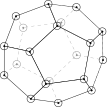
\includegraphics[width=0.5\textwidth]{../figures/hmvem/hmdof3d.pdf}
        \caption{$H^2$ 协调虚单元的自由度}
    \end{figure}
\end{minipage}
\end{frame}

\begin{frame}
\frametitle{多重调和方程}

\begin{definition}[多重调和方程]
  设区域 $\Omega = (0, 1)\times(0, 1)$,考虑如下多重调和方程:
  $$
  \left\{
  \begin{aligned}
      (-\Delta)^m u + c u & = f \quad \text{在 } \Omega\\
      \frac{\partial^j u}{\partial \boldsymbol{n}^j} & = 0 \quad \text{在 } \partial\Omega,~
      j = 0, 1, \dots, m-1.
  \end{aligned}
  \right.
  $$
\end{definition}

\begin{definition}[变分形式]
  寻找 $u \in H_0^m(\Omega)$,使得对任意 $v \in H_0^m(\Omega)$,
  $$
  (\nabla^m u, \nabla^m v) + c(u, v) = (f, v),
  $$
  其中 $f \in L^2(\Omega)$,$c \geq 0$ 为常数。
\end{definition}
\end{frame}

\begin{frame}
\frametitle{多重调和方程的虚单元法}

\begin{definition}[虚单元法 (VEM)]
  设 $\mathcal{T}_h$ 为 $\Omega$ 上的多面体剖分,定义虚单元空间:
  $$
  V_h := \{v_h \in H_0^m(\Omega): v_h|_K \in V_k^m(K), ~\forall K \in \mathcal{T}_h\}.
  $$
  多重调和方程的虚单元法为:
  {\bf 找到 $u_h \in V_h$,使得}
  $$
  a_h(u_h, v_h) = \langle f, v_h \rangle \quad \forall~v_h \in V_h,
  $$
  {\bf 其中}
  $$
  \langle f, v_h \rangle := \sum_{K \in \mathcal{T}_h}(f, Q_k^K v_h)_K, \quad
  a_h(u_h, v_h) := \sum_{K \in \mathcal{T}_h} a_{h,K}(u_h, v_h),
  $$
  $$
  \begin{aligned}
  a_{h,K}(u_h, v_h) :=&\, (\nabla^m \Pi_k^K u_h, \nabla^m \Pi_k^K v_h)_K
  + S_K(u_h - \Pi_k^K u_h, v_h - \Pi_k^K v_h) \\
  &+ c(Q_k^K u_h, Q_k^K v_h)_K.
  \end{aligned}
  $$
\end{definition}

\end{frame}

\begin{frame}
\frametitle{稳定化项与性质}

\begin{definition}[稳定化项]
  \footnotesize{
  $$
  S_K(w, v) := \sum_{r=1}^{n} \sum_{F \in \mathcal{F}^{r}(K)} \sum_{\substack{\alpha \in A_r \\ |\alpha| \leq m-1}} 
  h_K^{r + 2|\alpha| - 2m}
  \left(Q_{k - 2m + |\alpha|}^{F} \frac{\partial^{|\alpha|} w}{\partial \boldsymbol{n}_F^{\alpha}},
        Q_{k - 2m + |\alpha|}^{F} \frac{\partial^{|\alpha|} v}{\partial \boldsymbol{n}_F^{\alpha}}\right)_F
  $$
  }
\end{definition}

\begin{lemma}[稳定化项等价性]
  $$
  S_K(v - \Pi_k^K v, v - \Pi_k^K v) \eqsim |v - \Pi_k^K v|_{m, K}^2
  \quad \forall~v \in V_k^m(K).
  $$
\end{lemma}

\begin{lemma}[强制性]
  $$
  a_{h,K}(w, v) \lesssim (|w|_{m, K} + \|w\|_{0, K}) (|v|_{m, K} + \|v\|_{0, K})
  \quad \forall~w, v \in V_k^m(K),
  $$
  $$
  a_h(v_h, v_h) \eqsim |v_h|_m^2 \quad \forall~v_h \in V_h.
  $$
\end{lemma}

\end{frame}


\begin{frame}
\frametitle{误差估计}
\begin{theorem}\label{errorestimate}
设 $u \in H^s(\Omega) \cap H_0^m(\Omega)$ 是多重调和方程的真解,$u_h \in V_h$ 
是虚单元方法的数值解,且网格满足适当假设,
$f \in H^m(\mathcal{T}_h)$。则有如下误差估计:
$$
|u - u_h|_m \lesssim h^{\min\{s, k+1\} - m} |u|_{\min\{s, k+1\}} + \textrm{osc}_h(f),
$$
$$
|u - \Pi_h u_h|_{m, h} \lesssim h^{\min\{s, k+1\} - m} |u|_{\min\{s, k+1\}} + \textrm{osc}_h(f),
$$
其中
$$
\textrm{osc}_h^2(f) := \sum_{K \in \mathcal{T}_h} h_K^{2m} \|f - Q_k^K f\|_{0, K}^2.
$$
\end{theorem}
\end{frame}

\begin{frame}
  \frametitle{FEALPy数值算例一:双调和方程}
  考虑区域 $\Omega = (0, 1)\times(0, 1)$ 上的双调和方程:
  $$
  \left\{
  \begin{aligned} 
      \Delta^2 u + 2u & = f, \quad \text{在 } \Omega \\
      \frac{\partial^j u}{\partial \boldsymbol{n}^j} & = 0, \quad \text{在 } \partial\Omega,\ j = 0, 1
  \end{aligned}
  \right.
  $$
  精确解为 $u = \sin^2(\pi x)\sin^2(\pi y)$。

\begin{figure}[htb p]
\centering
\begin{minipage}[t]{0.49\linewidth}
\centering
\includegraphics[width=4cm]{../figures/convex.pdf}
\captionsetup{font={small}}
\caption{凸多边形网格 $\mathcal{T}_0$}
\end{minipage}%
\begin{minipage}[t]{0.49\linewidth}
\centering
\includegraphics[width=4cm]{../figures/nonconvex.pdf}
\captionsetup{font={small}}
\caption{非凸多边形网格 $\mathcal{T}_1$}
\end{minipage}
\end{figure}
\end{frame}

\begin{frame}
  \frametitle{双调和方程数值结果}
\begin{figure}[htbp]
\centering
\begin{minipage}[t]{0.49\linewidth}
\centering
\includegraphics[width=5cm]{../figures/H2_convex.pdf}
\end{minipage}%
\begin{minipage}[t]{0.49\linewidth}
\centering
\includegraphics[width=5cm]{../figures/H2_nonconvex.pdf}
\end{minipage}
\caption{双调和方程在凸网格 $\mathcal{T}_0$(左)和非凸网格 $\mathcal{T}_1$(右)上的误差 $|u - \Pi_h u_h|_{2, h}$,$m=2$,$k=2, 3, 4, 5$。}
\label{fig:H2error}
\end{figure} 
\end{frame}

\begin{frame}
    \frametitle{FEALPy数值算例二:三调和方程}
  考虑区域 $\Omega = (0, 1)\times(0, 1)$ 上的三调和方程:
  $$
  \left\{
  \begin{aligned}
      -\Delta^3 u + 2u & = f, \quad \text{在 } \Omega \\
      \frac{\partial^j u}{\partial \boldsymbol{n}^j} & = 0, \quad \text{在 } \partial\Omega,\ j = 0, 1, 2
  \end{aligned}
  \right.
  $$
  精确解为 $u = \sin^3(\pi x)\sin^3(\pi y)$。

\begin{figure}[htbp]
\centering
\begin{minipage}[t]{0.49\linewidth}
\centering
\includegraphics[width=4cm]{../figures/convex.pdf}
\captionsetup{font={small}}
\caption{凸多边形网格 $\mathcal{T}_0$}
\end{minipage}%
\begin{minipage}[t]{0.49\linewidth}
\centering
\includegraphics[width=4cm]{../figures/nonconvex.pdf}
\captionsetup{font={small}}
\caption{非凸多边形网格 $\mathcal{T}_1$}
\end{minipage}
\end{figure}
\end{frame}

\begin{frame}
    \frametitle{三调和方程数值结果}
\begin{figure}[htbp]
\centering
\begin{minipage}[t]{0.49\linewidth}
\centering
\includegraphics[width=5cm]{../figures/H3_convex.pdf}
\end{minipage}%
\begin{minipage}[t]{0.49\linewidth}
\centering
\includegraphics[width=5cm]{../figures/H3_nonconvex.pdf}
\end{minipage}
\caption{三调和方程在凸网格 $\mathcal{T}_0$(左)和非凸网格 $\mathcal{T}_1$(右)上的误差 $|u - \Pi_h u_h|_{3, h}$,$m=3$,$k=3, 4, 5, 6$。}
\label{fig:H3error}
\end{figure}
\end{frame}


\section{无稳定项虚单元方法}
\begin{frame}
\frametitle{求解 Poisson 方程的虚单元方法}
给定虚单元空间 $V_h$,虚单元方法的目标是寻找 $u_h \in V_h$,使得:
$$
a_h(u_h, v_h) = (f, v_h) \quad \forall v_h \in V_h,
$$
其中离散双线性形式 $a_h$ 定义为:
$$
a_h(u_h, v_h) = \sum_{K \in \mathcal{T}_h} a_h^K(u_h, v_h)
$$
$$
a_h^K(u_h, v_h) = \int_K \nabla \Pi_h^K u_h \cdot \nabla \Pi_h^K v_h \, \mathrm{d}x + \highlightit{S_h^K(u_h - \Pi_h^K u_h, v_h - \Pi_h^K v_h)}.
$$
其中稳定项 $S_h^K$ 需要满足:
$$
c_* |v|_{1, K}^2 \leq S_h^K(v, v) \leq C_* |v|_{1, K}^2 \quad \forall v \in 
V_h^K \cap \mathrm{ker}(\Pi_h^K).
$$
\end{frame}

\begin{frame}
\frametitle{无稳定项虚单元方法}

\begin{minipage}[b]{0.6\linewidth}
\uncover<1->{
\small{
\textbf{目标}:寻找一个合适的空间 $W_h^K$,使得:
\begin{itemize}
    \item 可以计算从 $ \nabla V_h^K$ 到 $ W_h^K $ 的投影 $Q^K$;
    \item $ \|Q^K \nabla v\| \eqsim \|\nabla v\| \quad \forall v \in V_h^K $。
\end{itemize}
\vspace{10pt}
}
\uncover<2->{
\textbf{方法}:

将多面体 $K$ 划分为一个单纯形网格 $\mathcal{T}_K$,在该网格上构造 $k$ 阶的 BDM 元空间 $\tilde{W}_h^k$,然后定义:
$$
W_h^{k-1} = \{\boldsymbol{v} \in \tilde{W}_h^{k-1}: \mathrm{div} \boldsymbol{v} \in
\mathbb{P}_{k-2}(K)\}.
$$
这样,从 $ \nabla V_h^K $ 到 $W_h^K$ 的 $L^2$ 正交投影 $Q^K$ 可通过以下公式计算:
$$
\begin{aligned}
(Q^K \nabla v, \boldsymbol{w})_K & = (\nabla v, \boldsymbol{w})_K\\
& = (v, \mathrm{div} \boldsymbol{w})_K + \langle v, \boldsymbol{w} \cdot 
\boldsymbol{n}\rangle_{\partial K}.
\end{aligned}
$$
}
}
\end{minipage}
\hfill
\begin{minipage}[b]{0.36\linewidth}
    \centering
    \uncover<2->
{
    \begin{figure}[htpb]
        \centering
        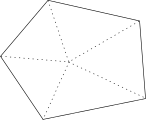
\includegraphics[width=0.75\textwidth]{../figures/splite_polygon.pdf}
        \caption{将多边形 $K$ 拆分三角形网格.}
    \end{figure}
}
\vspace{45pt}
\end{minipage}
\end{frame}

\begin{frame}
  \frametitle{网格条件}
  要求网格 $\mathcal{T}_h$ 满足以下条件:
  \begin{itemize}
    \item 对于任意单元 $K \in \mathcal{T}_h$ 和其 $r$ 维面 $F \in \mathcal{F}_h^r$,其中 $1 \leq r \leq d-1$,单元 $K$ 关于某个半径为 $\rho_K$ 的球是星形的,且 $\rho_K / h_K$ 有下界。
    \item 对于任意单元 $K \in \mathcal{T}_h$,存在一个准一致的单纯形网格 $\mathcal{T}_K$ 对其进行剖分,且 $\cup_{K \in \mathcal{T}_h} \mathcal{T}_K$ 构成一个形状规则的单纯形网格。
  \end{itemize}
  \vspace{10pt}
\begin{minipage}[b]{0.49\linewidth}
    \begin{figure}[htpb]
      \centering
      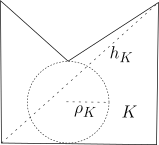
\includegraphics[width=0.55\textwidth]{../figures/star-shaped.pdf}
      \caption{星形区域示意图}
    \end{figure}
\end{minipage}
\hfill
\begin{minipage}[b]{0.49\linewidth}
    \centering
    \begin{figure}[htpb]
        \centering
        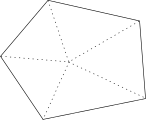
\includegraphics[width=0.55\textwidth]{../figures/splite_polygon.pdf}
        \caption{准一致单纯形剖分}
    \end{figure}
\end{minipage}
\end{frame}
\begin{frame}
    \frametitle{有限元微分 $d-2$ 形式}
对于每个 $T \in \mathcal{T}_K$,取 $\mathbb{P}_k(T, \mathbb{K})$ 作为形函数空间,定义如下自由度:
$$
\begin{aligned}
((\bsn_{1}^{e})^{\mathsf{T}}\tau\bsn_{2}^{e},q)_{e}, & \quad q\in\mathbb{P}_{k}(e),\ e\in\mathcal{E}(T), \\
(\mathrm{div}_{F}(\tau\bsn),q)_{F}, & \quad q\in\mathbb{P}_{k-1}(F)/\mathbb{R},\ F\in\mathcal{F}(T), \\
(\tau\bsn,\bsq)_F, & \quad \bsq\in\mathbb{P}_{k-2}(F;\mathbb{K})\bsx,\ F\in\mathcal{F}(T), \\
(\operatorname{div}\tau,q)_{T}, & \quad q\in\mathbb{P}_{k-3}(T;\mathbb{K})\bsx, \\
(\tau,\bsq)_{T}, & \quad \bsq\in\mathbb{P}_{k-2}(T;\mathbb{K})\cap\ker(\bsx).
\end{aligned}
$$

定义 $d-2$ 形式有限元空间 $V^{d-2}_k$ 为:
$$
\begin{aligned}
V^{d-2}_k = \{\tau \in L^2(K; \mathbb{K}) : & \tau|_T \in \mathbb{P}_k(T, \mathbb{K}),\ \forall T \in \mathcal{T}_K, \\
& \text{前三类自由度在全局上是单值的} \}.
\end{aligned}
$$

\uncover<2->{
\small{
\highlightit{
当 $d = 2$ 时,$V^{d-2}_k$ 是 Lagrange 元;
当 $d = 3$ 时,$V^{d-2}_k$ 是 N\'ed\'elec 元。
}
}
}
\end{frame}

\begin{frame}
    \frametitle{$H(\mathrm{div})$ 协调有限元空间:BDM 元}
对于 $k \geq 2$,定义 BDM 元空间:
$$
V^{\mathrm{BDM}}_{k-1}(K) := \{\bsv \in H(\diver, K) : \bsv|_T \in
\mathbb{P}_{k-1}(T; \mathbb{R}^d),\ \forall T \in \mathcal{T}_K\}.
$$

在单纯形 $T$ 上的局部自由度为:
$$
\begin{aligned}
(v\cdot\bsn,q)_{F}, & \quad q\in\mathbb{P}_{k-1}(F),\ F\in\mathcal{F}(T), \\
(\diver v, q)_{T}, & \quad q\in\mathbb{P}_{k-2}(T)/\mathbb{R}, \\
(v, \bsq)_T, & \quad \bsq\in\mathbb{P}_{k-3}(T;\mathbb{K})\bsx.
\end{aligned}
$$

定义其迹零子空间:
$$
\mathring{V}_{k-1}^{\mathrm{BDM}}(K):=V_{k-1}^{\mathrm{BDM}}(K)\cap\bsH_{0}(\mathrm{div},K).
$$
\end{frame}

\begin{frame}
    \frametitle{$H(\mathrm{div})$ 协调有限元空间:RT 元}
当 $k=1$ 时,定义最低阶 RT 元空间:
$$
V^{\mathrm{RT}}(K) := \{\bsv \in H(\diver, K) : \bsv|_T \in
\mathbb{P}_{0}(T; \mathbb{R}^d) + \bsx\mathbb{P}_{0}(T),\ \forall T \in \mathcal{T}_K\}.
$$

在单纯形 $T$ 上的局部自由度为:
$$
(v\cdot\bsn,q)_{F}, \quad q\in\mathbb{P}_{0}(F),\ F\in\mathcal{F}(T)
$$

其迹零子空间定义为:
$$
\mathring{V}^{\mathrm{RT}}(K):=V^{\mathrm{RT}}(K)\cap\bsH_{0}(\mathrm{div},K).
$$
\end{frame}

\begin{frame}
    \frametitle{有限元复形}
    当 $k \geq 2$ 时,以下有限元复形是恰当的:
$$
\begin{aligned}
V_{k}^{d-2}(K) & \xrightarrow{\mathrm{div~skw}}
V_{k-1}^{\mathrm{BDM}}(K) \xrightarrow{\mathrm{div}} V_{k-2}^{L^{2}}(K)
\to 0, \\
V_{1}^{d-2}(K) & \xrightarrow{\mathrm{div~skw}}
V^{\mathrm{RT}}(K) \xrightarrow{\mathrm{div}} V_{0}^{L^{2}}(K)
\to 0, \\
\mathring{V}_{k}^{d-2}(K) & \xrightarrow{\mathrm{div~skw}}
\mathring{V}_{k-1}^{\mathrm{BDM}}(K) \xrightarrow{\mathrm{div}}
\mathring{V}_{k-2}^{L^{2}}(K) \to 0, \\
\mathring{V}_{1}^{d-2}(K) & \xrightarrow{\mathrm{div~skw}}
\mathring{V}^{\mathrm{RT}}(K) \xrightarrow{\mathrm{div}}
\mathring{V}_{0}^{L^{2}}(K) \to 0,
\end{aligned}
$$
其中:
$$
\begin{aligned}
V_{k-2}^{L^{2}}(K) &= \{\tau \in L^2(K; \mathbb{K}) : \tau|_T \in
\mathbb{P}_{k-2}(T),\ \forall T \in \mathcal{T}_K\},\\ 
\mathring{V}_{k-2}^{L^{2}}(K) &= V_{k-2}^{L^{2}}(K)/\mathbb{R}.
\end{aligned}
$$
\end{frame}

\begin{frame}
    \frametitle{$H(\mathrm{div})$ 协调宏单元空间 $V^{\mathrm{div}}_{k-1}$}
定义 $H(\mathrm{div})$ 协调的宏单元空间 $V^{\mathrm{div}}_{k-1}(K)$ 为:
$$
V^{\mathrm{div}}_{k-1}(K) := \{\bsv \in V^{BDM}_{k-1}(K) : \diver
\bsv \in \mathbb{P}_{k-2}(K)\}.
$$
当 $k=1$ 时,定义:
$$
V^{\mathrm{div}}_{0}(K) := \{\bsv \in V^{RT}(K) : \diver
\bsv \in \mathbb{P}_{0}(K)\}.
$$
以下复形是恰当的:
$$
\begin{aligned}
V_{k}^{d-2}(K) & \xrightarrow{\mathrm{div~skw}}
V^{\mathrm{div}}_{k-1}(K) \xrightarrow{\mathrm{div}}
\mathbb{P}_{\max\{k-2, 0\}}(K) \to 0
\end{aligned}
$$
根据有限元复形理论,可以将 $V^{\mathrm{div}}_{k-1}(K)$ 分解为:
$$
V^{\mathrm{div}}_{k-1}(K) = \mathrm{div~skw}V_{k}^{d-2}(K) \oplus 
(\boldsymbol{x-x}_K)\mathbb{P}_{\max\{k-2, 0\}}(K).
$$
\end{frame}

\begin{frame}
    \frametitle{$H(\mathrm{div})$ 协调宏单元子空间 $\mathbb{V}^{\mathrm{div}}_{k-1}$}
    由于 $V^{\mathrm{div}}_{k-1}$ 在单元 $K$ 的边界上不是多项式,我们取其子空间:
    $$
    \mathbb{V}^{\mathrm{div}}_{k-1}(K) := \{\bsv \in
        V^{\mathrm{div}}_{k-1}(K) :
        \bsv \cdot \bsn|_F \in \mathbb{P}_{k-1}(F),
    \forall F \in \mathcal{F}(K)\}.
    $$
    其自由度如下:
    $$
    \begin{aligned}
        (v\cdot\bsn,q)_{F}, & \quad
        q \in \mathbb{P}_{k-1}(F), F \in \mathcal{F}(K), \\
        (\diver v, q)_{K}, & \quad q \in \mathbb{P}_{\max\{k-2, 0\}}(K)/\mathbb{R}, \\
        (v, \bsq)_K, & \quad
        \bsq \in \diver \mathring{V}_k^{d-2}(K).
    \end{aligned}
    $$
    $\mathbb{V}_{k-1}^{\mathrm{div}}$ 中的函数满足以下范数等价关系:
    $$
    \|\bsv\|_{0, K} \eqsim h_K\|\diver \bsv\|_{0, K} + 
    \sup_{\psi \in \diver \mathring{V}_k^{d-2}(K)}\frac{(\bsv,
    \psi)_K}{\|\psi\|_{0, K}} + \sum_{F \in \mathcal{F}(K)}h_F^{1/2}\|v\cdot
    \bsn\|_{0, F}.
    $$
\end{frame}

\begin{frame}
\frametitle{非协调虚单元空间}
定义非协调虚单元空间:
$$
\begin{aligned}
    V_k(K) := \{v \in H^1(K): & \partial_n v|_{F} \in \mathbb{P}_{k-1}(F), 
        \forall F \in \mathcal{F}(K), \\
    & \Delta v \in \mathbb{P}_{k}(K),\\
    & (v-\Pi_k^K v, q)_K = 0 \quad \forall q \in
    \mathbb{P}_{k-2}^{\perp}(K)\}.
\end{aligned}
$$
其中 $\Pi_k^K$ 表示到 $\mathbb{P}_k(K)$ 的 $H^1$ 投影。
虚单元的自由度为:
$$
\begin{aligned}
    \frac{1}{|F|}(v, q)_{F}, & \quad q \in \mathcal{M}_{k-1}(F), \\
    \frac{1}{|K|}(v, q)_{K}, & \quad q \in \mathcal{M}_{k-2}(K), \\
\end{aligned}
$$
其中 $\mathcal{M}_{k-1}(F)$ 和 $\mathcal{M}_{k-2}(K)$ 分别为 $F$ 和 $K$ 上的标准化单项式基。
定义 $\nabla V_k(K)$ 到 $\mathbb{V}^{\mathrm{div}}_{k-1}(K)$ 的 $L^2$ 投影 $Q_{K, k-1}^{\mathrm{div}}$:
$$
(Q_{K, k-1}^{\mathrm{div}}\nabla v, \bsw)_K := (\nabla v,
\bsw)_K = -(v, \diver \bsw)_K + \langle v, \bsw 
\cdot \bsn\rangle_{\partial K}.
$$
\end{frame}

\begin{frame}
    \frametitle{非协调虚单元方法:范数等价性}
    \begin{lemma}
        以下的 Inf-Sup 条件成立:
        $$
        \|\nabla v\| \leq C \sup_{\bsw \in
        \mathbb{V}^{\mathrm{div}}_{k-1}(K)}\frac{(\nabla v,
        \bsw)_K}{\|\bsw\|} \quad \forall v \in V_k(K).
        $$
        其中常数 $C$ 与网格大小无关,仅依赖于多项式次数 $k$、空间维度 $d$、多面体的星形常数以及网格的拟一致性和形状正则性参数。
        
        以下的范数等价性成立:
        $$
        \|Q_{K, k-1}^{\mathrm{div}}\nabla v\|_{0, K} \eqsim \|\nabla v\|_{0, K} 
        \quad \forall v \in V_k(K).
        $$
    \end{lemma}
\end{frame}

\begin{frame}
\frametitle{无稳定化项非协调虚单元方法求解 Poisson 方程}
\small{
稳定化项虚单元方法为:寻找 $u_h \in V_k$ 满足
$$
a_h(u_h, v_h) = (f, Q_h v_h) \quad \forall v_h \in V_k,
$$
其中 $a_h$ 定义为:
$$
a_h(u_h, v_h) = \sum_{K \in \mathcal{T}_h} a_h^K(u_h, v_h),
$$
$$
a_h^K(u_h, v_h) = (Q_{K, k-1}^{\mathrm{div}}\nabla u_h, Q_{K,
k-1}^{\mathrm{div}}\nabla v_h)_K.
$$
单元上的离散双线性形式 $a_h^K$ 满足如下稳定性条件:
$$
c_* |v|_{1, K}^2 \leq a_h^K(v, v) \leq C_* |v|_{1, K}^2 \quad \forall v \in
V_k^K.
$$
\begin{theorem}
若 $u \in H^{k+1}(\Omega), f \in H^{k-1}(\Omega)$,则上述虚单元方法是稳定的,且有如下误差估计:
$$
|u - u_h|_{1, \Omega} \leq C h^{k}
(|u|_{k+1, \Omega} + |f|_{k-1, \Omega}).
$$
\end{theorem}
}
\end{frame}

\begin{frame}
\frametitle{协调虚单元方法:空间构造}
假设所有面都是单纯形。定义 $H^1$ 协调虚单元空间:
$$
\begin{aligned}
    V_k(K) := \{v \in H^1(K): & v|_{\partial K} \in H^1(\partial K), v|_F \in 
        \mathbb{P}_k(e), \forall e \in \mathcal{F}(K),
    \Delta v \in \mathbb{P}_{k}(K),\\
    & (v-\Pi_k^K v, q)_K = 0 \quad \forall q \in
    \mathbb{P}_{k-2}^{\perp}(K)\}.
\end{aligned}
$$
其中 $\Pi_k^K$ 是 $H^1$ 投影到 $\mathbb{P}_k(K)$ 上。
虚单元的自由度如下:
$$
\begin{aligned} 
    v(\delta), & \quad \delta \in \Delta_0(K), \\
    \frac{1}{|e|}(v, q)_{e}, & \quad q \in \mathcal{M}_{k-j-1}(e), \forall e \in
    \Delta_j(K), j = 1, \dots, d-1,\\
    \frac{1}{|K|}(v, q)_{K}, & \quad q\in \mathcal{M}_{k-2}(K), \\
\end{aligned}
$$
其中 $\mathcal{M}_{k-j-1}(e)$ 和 $\mathcal{M}_{k-2}(K)$ 分别是边和单元上的尺度单项式。
定义 $Q_{K, k-1}^{\mathrm{div}}$ 为 $\nabla V_k(K)$ 到
$\mathbb{V}^{\mathrm{div}}_{k}(K)$ 上的 $L^2$ 投影:
$$
(Q_{K, k}^{\mathrm{div}}\nabla v, \bsw)_K := (\nabla v,
\bsw)_K = -(v, \diver \bsw)_K + \langle v, \bsw 
\cdot \bsn\rangle_{\partial K}.
$$
\end{frame}

\begin{frame}
    \frametitle{协调虚单元方法:范数等价性}
    \begin{lemma}
        以下的 Inf-Sup 条件成立:
        $$
        \|\nabla v\| \leq C \sup_{\bsw \in
        \mathbb{V}^{\mathrm{div}}_{k}(K)}\frac{(\nabla v,
        w)_K}{\|\bsw\|} \quad \forall v \in V_k(K).
        $$
        其中常数 $C$ 与网格大小、$k$、空间维度 $d$、多面体的星形常数以及网格的拟一致性和形状正则性参数有关。
        
        以下的范数等价性成立:
        $$
        \|Q_{K, k}^{\mathrm{div}}\nabla v\|_{0, K} \eqsim \|\nabla v\|_{0, K} 
        \quad \forall v \in V_k(K).
        $$
    \end{lemma}
\end{frame}

\begin{frame}
    \frametitle{协调虚单元方法求解 Poisson 方程}
无稳定化项虚单元方法为:寻找 $u_h \in V_k$ 满足
$$
a_h(u_h, v_h) = (f, Q_h v_h) \quad \forall v_h \in V_k,
$$
其中 $a_h$ 定义为:
$$
a_h(u_h, v_h) = \sum_{K \in \mathcal{T}_h} a_h^K(u_h, v_h),
$$
$$
a_h^K(u_h, v_h) = (Q_{K, k}^{\mathrm{div}}\nabla u_h, Q_{K,
k}^{\mathrm{div}}\nabla v_h)_K.
$$
单元上的离散双线性形式 $a_h^K$ 满足如下稳定性条件:
$$
c_* |v|_{1, K}^2 \leq a_h^K(v, v) \leq C_* |v|_{1, K}^2 \quad \forall v \in
V_k^K.
$$
\begin{theorem}
若 $u \in H^{k+1}(\Omega), f \in H^{k-1}(\Omega)$,则上述虚单元方法是稳定的,且有如下误差估计:
$$
|u - u_h|_{1, \Omega} \leq C h^{k}
(|u|_{k+1, \Omega} + |f|_{k-1, \Omega}).
$$
\end{theorem}
\end{frame}

\begin{frame}
    \frametitle{实现:$\mathbb{V}^{\mathrm{div}}_{k-1}$ 的基函数构造}
    \begin{minipage}[b]{0.55\linewidth}
    \textbf{在二维情形下},
    空间 $\mathbb{V}^{\mathrm{div}}_{k-1}$ 可分解为:
    $$
    \mathbf{rot} V^{Lag}_k \oplus (\mathbf{x-x}_K)\mathbb{P}_{k-2}(K)。 
    $$
    因此可定义如下基函数集合:
    $$
    \mathbf{rot} \{\Phi^{Lag}_k/\phi_0\} \oplus (\mathbf{x-x}_K)
    \mathcal{M}_{k-2}(K)。
    $$
    其中 $\Phi^{Lag}_k$ 为 Lagrange 元空间的基函数,$\phi_0$
    表示对应于中心点的基函数。
\end{minipage}
\hfill
\begin{minipage}[b]{0.4\linewidth}
    \centering
    \begin{figure}[htpb]
        \centering
        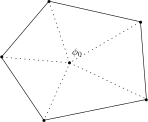
\includegraphics[width=0.8\textwidth]{../figures/lagrange_phi0.pdf}
        \caption{中心点上的 Lagrange 元基函数}
    \end{figure}
\vspace{5pt}
\end{minipage}
\end{frame}

\begin{frame}
\frametitle{FEALPy数值算例一:收敛性分析}
考虑以下二阶椭圆方程:
$$
\left\{
\begin{aligned}
    -\Delta u + 2u & = f \quad \Omega \\
    u & = 0 \quad \partial\Omega
\end{aligned}
\right.
$$
其中 $\Omega = (0, 1)\times(0, 1)$,已知精确解与右端项为:
$$
u = \sin(\pi x)\sin(\pi y), \quad f = (2\pi^2+2)\sin(\pi x)\sin(\pi y)。
$$

\begin{figure}[htbp]
\centering
\begin{minipage}[t]{0.49\linewidth}
\centering
\includegraphics[width=4cm]{../figures/convex.pdf}
\captionsetup{font={small}}
\caption{凸多边形网格 $\mathcal T_0$}
\end{minipage}%
\begin{minipage}[t]{0.49\linewidth}
\centering
\includegraphics[width=4cm]{../figures/nonconvex.pdf}
\captionsetup{font={small}}
\caption{非凸多边形网格 $\mathcal T_1$}
\end{minipage}%
\centering
\end{figure}
\end{frame}

\begin{frame}
\frametitle{FEALPy数值算例一:收敛性分析}
选取 $k = 1, 2, 5$,在 SFNCVEM 与 SFCVEM 方法中进行测试。
下图展示了 SFNCVEM 方法在网格 $\mathcal T_0$ 和 $\mathcal T_1$ 上的数值结果。
可观察到误差 $\|u - Q_h u_h\|_0=O(h^{k+1})$ 以及 $\|\nabla u -
Q_{h}\nabla_h u_h\|_0=O(h^{k})$。
\begin{figure}[htbp]
\centering
\begin{minipage}[t]{0.49\linewidth}
\centering
\includegraphics[width=5.5cm]{../figures/stabfree/ncvem_convex.pdf}
\end{minipage}%
\begin{minipage}[t]{0.49\linewidth}
\centering
\includegraphics[width=5.5cm]{../figures/stabfree/ncvem_nonconvex.pdf}
\end{minipage}%
\centering
\caption{SFNCVEM 方法在凸网格 $\mathcal T_0$(左)和非凸网格 $\mathcal T_1$(右)上,
不同阶次 $k=1,2,5$ 的误差 $\|u - Q_h u_h\|_0$ 与 $\|\nabla u - Q_{h}\nabla_h u_h\|_0$。}
\label{fig:rate1}
\end{figure}
\end{frame}

\begin{frame}
\frametitle{FEALPy数值算例一:收敛性分析}
下图展示了 SFCVEM 方法在不同网格上的数值结果,
同样满足误差估计 $\|u - Q_h u_h\|_0=O(h^{k+1})$ 与
$\|\nabla u - Q_{h}\nabla u_h\|_0=O(h^{k})$。

\begin{figure}[htbp]
\centering
\begin{minipage}[t]{0.49\linewidth}
\centering
\includegraphics[width=5.5cm]{../figures/stabfree/cvem_convex.pdf}
\end{minipage}%
\begin{minipage}[t]{0.49\linewidth}
\centering
\includegraphics[width=5.5cm]{../figures/stabfree/cvem_nonconvex.pdf}
\end{minipage}%
\centering
\caption{SFCVEM 方法在凸网格 $\mathcal T_0$(左)和非凸网格 $\mathcal T_1$(右)上,
不同阶次 $k=1,2,5$ 的误差 $\|u - Q_h u_h\|_0$ 与 $\|\nabla u - Q_{h}\nabla u_h\|_0$。}
\label{fig:rate2}
\end{figure}
\end{frame}

\begin{frame}
    \frametitle{FEALPy数值算例二:条件数分析}
我们构造了如下图所示的三种不同的六边形,并在 $k=3$ 的情况下,计算了四种虚单元方法对应的局部刚度矩阵的特征值。
\begin{figure}[htbp]
\centering
\begin{subfigure}[t]{0.32\linewidth}
    \centering
    \includegraphics[width=1in]{../figures/stabfree/hexagon0.pdf}
\end{subfigure}%
\begin{subfigure}[t]{0.32\linewidth}
    \centering
    \includegraphics[width=1in]{../figures/stabfree/hexagon1.pdf}
\end{subfigure}%
\begin{subfigure}[t]{0.32\linewidth}
    \centering
    \includegraphics[width=0.9in]{../figures/stabfree/hexagon2.pdf}
\end{subfigure}
\caption{左:规则六边形;中:由规则六边形扰动得到的拟规则六边形;右:带有两个悬挂节点的方形。}
\label{fig:all}
\end{figure}
\end{frame}

\begin{frame}
    \frametitle{FEALPy数值算例二:条件数分析}
我们进一步展示不同六边形上的局部刚度矩阵的最小非零特征值、最大特征值以及条件数。从中可以看出,四种虚单元方法的这些数值是相似的。
\only<1>{
\begin{table}[htbp]
\centering
\caption{规则六边形上特征值与条件数的比较}
\begin{tabular}{c|ccc}
\hline
\textbf{方法} & \textbf{最大特征值} & \textbf{最小特征值} & \textbf{条件数} \\ \hline
NCVEM & 975.5693189 & 0.309674737 & 3150.303211 \\ \hline
CVEM & 1012.488116 & 0.297206358 & 3406.683909 \\ \hline
SFNCVEM & 992.5956147 & 0.318932029 & 3112.248147 \\ \hline
SFCVEM & 1011.173331 & 0.298509692 & 3387.405362 \\
\hline
\end{tabular}
\end{table}
}
\only<2>{
\begin{table}[htbp]
\centering
\caption{拟规则六边形上特征值与条件数的比较}
\begin{tabular}{c|ccc}
\hline
\textbf{方法} & \textbf{最大特征值} & \textbf{最小特征值} & \textbf{条件数} \\ \hline
NCVEM   & 935.2883848 & 0.279027715 & 3351.955143 \\ \hline
CVEM    & 1014.672395 & 0.257370621 & 3942.456177 \\ \hline
SFNCVEM & 997.4831245 & 0.282126359 & 3535.589964 \\ \hline
SFCVEM  & 1047.876056 & 0.258970708 & 4046.311124 \\
\hline
\end{tabular}
\end{table}
}
\only<3>{
\begin{table}[htbp]
\centering
\caption{带悬挂节点的方形上特征值与条件数的比较}
\begin{tabular}{c|ccc}
\hline
\textbf{方法} & \textbf{最大特征值} & \textbf{最小特征值} & \textbf{条件数} \\ \hline
NCVEM   & 941.8571938 & 0.21069027  & 4470.340249 \\ \hline
CVEM    & 1046.755495 & 0.200435123 & 5222.4155 \\ \hline
SFNCVEM & 986.5963357 & 0.212761106 & 4637.108513 \\ \hline
SFCVEM  & 1061.651989 & 0.202074633 & 5253.761808 \\
\hline
\end{tabular}
\end{table}
}
\end{frame}

\begin{frame}
\frametitle{FEALPy数值算例三:计算时间}
我们在凸多边形网格上进行了实验。下表展示了刚度矩阵的构造时间。可以看出,NCVEM、CVEM 和 SFNCVEM 的构造时间相近,而 SFCVEM 由于需要投影到高次多项式空间,其计算时间更长。
\only<1>{
\begin{table}[htbp]
\centering
\caption{不同 $k$ 值下四种 VEM 方法的刚度矩阵构造时间($h = 0.2$)}
\begin{tabular}{c|cccc}
\hline
\textbf{k} & \textbf{2} & \textbf{4} & \textbf{8} & \textbf{10} \\ \hline
SFCVEM & 0.053684235 & 0.144996881 & 1.468627453 & 2.603836536 \\ \hline
SFNCVEM & 0.022516727 & 0.065697193 & 0.806378841 & 1.554260015 \\ \hline
CVEM & 0.021185875 & 0.059809923 & 0.600241184 & 1.160929918 \\ \hline
NCVEM & 0.0213027   & 0.061014891 & 0.596506596 & 1.129639149 \\
\hline
\end{tabular}
\end{table}
}
\only<2>{
\begin{table}[htbp]
\centering
\caption{固定 $k=5$,不同 $h$ 值下四种 VEM 方法的刚度矩阵构造时间}
\begin{tabular}{c|cccc}
\hline
\textbf{h} & \textbf{1} & \textbf{0.25} & \textbf{0.0625} & \textbf{0.03125} \\ \hline
SFCVEM & 0.039689541 & 0.199015379 & 1.74412179 & 4.75462532 \\ \hline
SFNCVEM & 0.018287182 & 0.100006819 & 0.81251812 & 2.465409517 \\ \hline
CVEM & 0.018686771 & 0.087426662 & 0.781031132 & 1.983617783 \\ \hline
NCVEM & 0.018309593 & 0.096345425 & 0.767129898 & 2.159288645 \\
\hline
\end{tabular}
\end{table}
}
\end{frame}

\section{带有 Lipschitz 界面的时谐 Maxwell 方程的虚单元方法}
\begin{frame}
  \frametitle{界面问题}
  \begin{figure}[htpb]
      \centering
      \begin{subfigure}[t]{0.49\linewidth}
          \centering
          \includegraphics[width=0.6\textwidth]{../figures/big.png}
          \caption{发电机二维模型。}
      \end{subfigure}%
      \begin{subfigure}[t]{0.49\linewidth}
          \centering
          \includegraphics[width=0.8\textwidth]{../figures/bbig.png}
          \caption{超构透镜模型。}
      \end{subfigure}
  \caption{界面问题几何模型。}
  \end{figure}

  \mycomment{虚单元方法可以在多边形网格上使用的特点可以在界面问题中应用,
      界面问题是指材料的参数在整个区域上不均匀分布的问题,反应在 PDE 上就是
      某些系数在计算区域上不连续。这种问题需要网格拟合界面,
      如在电磁问题中,很多元件的尺寸都很小,这对与界面拟合网格的生成很困难。
  但使用虚单元方法的话,可以有简单的方法来生成界面拟合网格。}
\end{frame}


\begin{frame}
    \frametitle{界面拟合网格生成}
\begin{figure}[htbp]
\begin{subfigure}[t]{0.49\linewidth}
    \centering
    \includegraphics[width=1.2in]{../figures/movingmaxwell/interface_half_cricle.pdf}
\end{subfigure}
\begin{subfigure}[t]{0.49\linewidth}
    \centering
    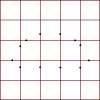
\includegraphics[width=1.2in]{../figures/movingmaxwell/cut_point.pdf}
\end{subfigure}
\end{figure}

\begin{figure}[htbp]
\begin{subfigure}[t]{0.49\linewidth}
    \centering
    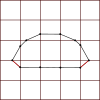
\includegraphics[width=1.2in]{../figures/movingmaxwell/cut_mesh_0.pdf}
\end{subfigure}
\begin{subfigure}[t]{0.49\linewidth}
    \centering
    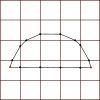
\includegraphics[width=1.2in]{../figures/movingmaxwell/cut_mesh_1.pdf}
\end{subfigure}
\end{figure}

\mycomment{这样做会带来一些问题,会切割出一些形状很差的单元,需要对这种情况进行分析。
那么这样的算法在电磁问题的数值模拟中是有意义的。}

\end{frame}

\begin{frame}
\frametitle{Maxwell 方程}
设$\Omega$为 $\mathbb{R}^3$ 中的单连通区域,考虑 Maxwell 方程组:
$$
\left\{
\begin{aligned}
  \curl \boldsymbol{H} & = \partial_t \boldsymbol{D} +
  \boldsymbol{J} \quad \quad & \text{Maxwell-Amp\'ere 方程,} \\
  \curl \boldsymbol{E} & = -\partial_t \boldsymbol{B}
  & \text{Faraday 方程,} \\
  \diver \boldsymbol{D} & = \rho & \text{Gauss 电场方程,} \\
  \diver \boldsymbol{B} & = 0 & \text{Gauss 磁场方程,}
\end{aligned}
\right.
$$
其中,$\boldsymbol{H}$是磁场,$\boldsymbol{E}$是电场,
$\boldsymbol{B}$是磁通密度,$\boldsymbol{D}$是电通量密度,
$\boldsymbol{J}$是电流密度,$\rho$是电荷密度。且满足:
$$
\bsB = \mu \bsH, \quad \bsD = \epsilon \bsE,
\quad \bsJ = \sigma \bsE + \bsJ_s
$$
其中,$\epsilon$是介电常数,$\mu$是磁导率,$\sigma$是电导率,$\bsJ_s$是源电流。
Maxwell 可化简为仅包含 $\boldsymbol{E}$ 的方程:
$$
\curl \mu^{-1}\curl \boldsymbol{E} + \partial_t^2 \epsilon \boldsymbol{E} 
- \partial_t \sigma \boldsymbol{E} = \partial_t \boldsymbol{J}_s
$$
\end{frame}

\begin{frame}
    \frametitle{时谐 Maxwell 方程}
当 $\bsE$ 是时谐的,可消去 Maxwell 方程中的时间变量,得到
$$
\curl \mu^{-1}\curl \boldsymbol{\bsu} - \omega^2(\epsilon + i\sigma/\omega)
\boldsymbol{\bsu} = \bssf.
$$
其中 $\bsu = \bsE(\cdot, 0)e^{i\omega t}$,
$\bssf = i\omega\bsJ_s(\cdot, 0) e^{i\omega t}$,$\omega$ 是固定的角频率,
$i = \sqrt{-1}$ 是虚数单位。考虑如下情况:
\begin{itemize}
    \item 电磁波是 TE 波,即 $E_z = 0$,问题退化为二维问题。
    \item $\sigma = 0$,$\omega^2 \epsilon > 0$。
    \item 界面 $\Gamma$ 非光滑,将计算区域 $\Omega$ 划分为两个区域
    $\Omega^+$ 和 $\Omega^-$。
    \item $\epsilon$ 和 $\mu$ 在每个区域内是常数。
\end{itemize}
这种情况下问题可写为:
$$
\brot \alpha \rot \boldsymbol{u} - \beta 
\boldsymbol{u} = \bssf,
$$
其中 $\brot$ 是旋度算子,$\alpha = \mu^{-1}$, $\beta = \omega^2\epsilon>0$。

\end{frame}

\begin{frame}
    \frametitle{时谐 Maxwell 方程界面问题}
\begin{minipage}[b]{0.6\linewidth}
\small
    考虑如下时谐 Maxwell 方程:
    $$
    \left\{
    \begin{aligned}
        \brot \alpha \rot \boldsymbol{u} - \beta \boldsymbol{u} & = \boldsymbol{f} \quad
        \Omega\\
        \bsu\times \bsn & = 0 \quad \partial\Omega
    \end{aligned}
    \right.
    $$
    其中 $\bssf \in \bsH(\diver^0; \Omega), \alpha > 0, \beta > 0$ 是分片常数:
    $$
    \alpha = \left\{
    \begin{aligned}
        \alpha_1 \quad & \text{in } \Omega^+,\\
        \alpha_2 \quad & \text{in } \Omega^-,
    \end{aligned}
\right.\quad
\beta = \left\{
\begin{aligned}
    \beta_1 \quad & \text{in } \Omega^+,\\
    \beta_2 \quad & \text{in } \Omega^-,
\end{aligned}
\right.
    $$
    界面条件为:
$$
\begin{aligned}
[\mathbf{u}\cdot\mathbf{t}]_{\Gamma} :=
(\mathbf{u}^+\cdot\mathbf{t}-\mathbf{u}^-\cdot\mathbf{t})|_{\Gamma} = 0\\
[\alpha \rot \mathbf{u}]_{\Gamma} := (\alpha \rot \mathbf{u}^+
- \alpha \rot \mathbf{u}^-)|_{\Gamma} = 0.
\end{aligned}
$$
变分问题为:找到 $\bsu \in \bsH_0(\rot;\Omega)$ 使得
$$
\begin{aligned}
    a(\bsu, \bsv) := (\alpha \rot \bsu, \rot \bsv) - (\beta \bsu, \bsv) =
    (\bssf, \bsv) \quad \forall \bsv \in \bsH_0(\rot;\Omega),
\end{aligned}
$$
\end{minipage}
\hfill
\begin{minipage}[b]{0.38\linewidth}
    \centering
    \begin{figure}[htpb]
        \centering
        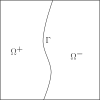
\includegraphics[width=0.8\textwidth]{../figures/interface_prob.pdf}
        \caption{界面问题求解区域.}
    \end{figure}
\vspace{10pt}
\end{minipage}
\end{frame}

\begin{frame}
    \frametitle{界面假设}
\begin{assumption}[界面假设]
界面满足以下条件:
\begin{itemize}
\item[(I1)]\label{asp:I1} 界面不与自身相交;
\item[(I2)]\label{asp:I2} 正则性质:存在常数$c_0$使得
\begin{equation}
\label{Dregular}
|B(\bsx,r)\cap \Omega^{\pm}| \ge c_0 r^2 ~~~ \forall \bsx \in \Omega^{\pm}, ~~ r\in[0,1],
\end{equation}
其中$B(\bsx,r)$表示以$\bsx$为中心、$r$为半径的球。
\end{itemize}
\end{assumption}
\begin{figure}[htpb]
    \centering
    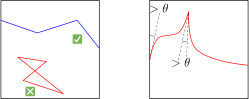
\includegraphics[width=0.5\textwidth]{../figures/maxwell/interface_assumption.pdf}
    \caption{界面不能与自身相交(左图);界面夹角不能太小(右图)。}
\end{figure}
\end{frame}

\begin{frame}
\small
\begin{lemma}
在假设 \hyperref[asp:I1]{(I1)} 下,椭圆界面问题:
\begin{equation}
\begin{split}
\label{H1eqn}
& \diver(a\nabla u) = f ~~ \text{in} ~~ \Omega, ~~~~ [u]_{\Gamma} =0, ~ [a\nabla
u\cdot\bsn]_{\Gamma}=0 ~ \text{on} ~ \Gamma,\\
& u=0 ~~ \text{or} ~~ a\nabla u \cdot \bsn =0 ~ \text{on} ~~ \partial\Omega,
\end{split}
\end{equation}
解$u\in H^{1+\theta}_0(\Omega^{\pm})$,$\theta\in(1/2,1]$。
\end{lemma}

\begin{lemma}
\label{lem_embd_1}
在假设 \hyperref[asp:I1]{(I1)} 条件下,存在 $\theta\in(1/2,1]$,使得
\begin{equation}
\label{lem_embd_1_eq0}
\bsH_0(\rot;\Omega)\cap \bsH(\beta, \diver;\Omega) \hookrightarrow \bsH^{\theta}(\Omega^{\pm}).
\end{equation}
此外,
如果 $\Omega$ 是星形的,则
对于任意 $\bsu\in \bsH_0(\rot;\Omega)\cap \bsH(\beta, \diver;\Omega)$,
那么有:
\begin{equation}
  \label{lem_embd_1_eq01}
  \| \bsu \|_{0,\Omega} 
  \le 2 \sqrt{\varpi}  h^2_{\Omega}|\Omega|^{-1/2} \|\rot \bsu \|_{0,\Omega} 
  + \beta_{\min}^{-1} ( \sqrt{\pi} j_0)^{-1} |\Omega|^{1/2} \|\diver(\beta \bsu) \|_{0,\Omega},
  \end{equation}
其中 $h_{\Omega}$ 是 $\Omega$ 的直径,$|\Omega|$ 是面积,
$\beta_{\max(\min)}=\max(\min)\{\beta^+,\beta^-\}$,
$\varpi = \beta_{\max}/\beta_{\min}$。
%如果 $\Omega$ 是凸多边形或具有光滑边界,则 $\theta=1$。
\end{lemma}
\end{frame}

%\begin{frame}
%\frametitle{方程解的存在唯一性}
%\small
%\begin{assumption}[特征值假设]
%\label{assum_eigen}
%$\beta$不是$\brot\alpha\rot$算子的特征值,即不存在$\bsu \in
%\bsH_0(\rot;\Omega)$使得
%$$
%\brot\alpha\rot \bsu = \beta \bsu.
%$$
%\end{assumption}
%\begin{remark}
%假设 $\Omega$ 关于半径为 $r_{\Omega}\ge \nu h_{\Omega}$ 的球是星形的,其中 $\nu\in(0,1)$。  
%那么当 $\bsu \in \bsH_0(\rot;\Omega)\cap \bsH(\beta, \diver^0;\Omega)$ 时,
%$$
%\| \bsu \|_{0,\Omega} \le 2 \sqrt{\varpi} h^2_{\Omega}|\Omega|^{-1/2} \| \rot\bsu \|_{0,\Omega} 
%\le \sqrt{\varpi/\pi} \nu^{-1} h_{\Omega} \| \rot\bsu \|_{0,\Omega}.
%$$
%因此,如果我们固定 $\nu$ 并使 $\Omega$ 足够小,使得
%$h_{\Omega} <  \nu \sqrt{ \frac{\alpha_{\min}}{\beta_{\max}} \frac{\pi}{\varpi}
%}$,
%则有
%\begin{equation}
%  \label{dom_small_eq2}
%\| \sqrt{\alpha} \rot \bsu \|^2_{0,\Omega} \ge \alpha_{\min} \| \rot \bsu \|^2_{0,\Omega} > \beta_{\max} \| \bsu \|^2_{0,\Omega},
%\end{equation}
%这保证了特征值假设的成立。
%\end{remark}
%\end{frame}

\begin{frame}
\frametitle{网格假设}
\begin{assumption}[薄带假设]
\label{interf_eps}
存在与网格无关、仅依赖于$\Gamma$的常数$\epsilon>0$,使得
\begin{equation}
\label{interf_eps_eq}
(\Omega^+_h\cap \Omega^-)\cup (\Omega^-_h\cap \Omega^+) \subseteq
\Omega^{\Gamma}_{\epsilon h^2} := \{\bsx \in \Omega : \mathrm{dist}(\bsx, \Gamma) <
\epsilon h^2\},
\end{equation}
\end{assumption}

\begin{figure}[h]
\centering
\begin{subfigure}{.3\textwidth}
    \includegraphics[width=1.05in]{../figures/maxwell/interfelem1}
\label{fig:interfelem1}
\end{subfigure}
%%
\begin{subfigure}{.3\textwidth}
    \includegraphics[width=1.05in]{../figures/maxwell/interfelem3}
\label{fig:interfelem2}
\end{subfigure}
%%
\begin{subfigure}{.3\textwidth}
    \includegraphics[width=1.05in]{../figures/maxwell/interfelem2}
\label{fig:interfelem3}
\end{subfigure}
%%
\caption{左:界面(红色)将单元$K$切割为两个子单元;通过连接交点构造近似线段$\Gamma^K_h$(蓝色)。
中:分段光滑界面曲线的多边形近似$\Gamma^K_h$。
右:$\Omega^{\pm}$与$\Omega^{\pm}_h$的不匹配区域,该区域包含在薄带$\Omega_{\epsilon
h^2}$中.}
\label{fig:interfelem}
\end{figure}

\end{frame}

\begin{frame}
    \begin{assumption}[虚拟网格假设]
\label{assump_vmesh}多边形 $K$ 的顶点个数与边个数一致有界。
存在局部“虚拟网格”$\mathcal{T}_K$满足:
\begin{itemize}
\item[(L1)] \label{asp:polygonL1} 最大角条件:$\mathcal T_h(K)$中所有三角形的角度均不超过$\theta_M< \pi$。
\item[(L2)] \label{asp:polygonL2} 短内边条件:存在$d_1, d_2 > 0$,使得对于任何内边$e$,要么$h_e \ge d_1 h_K$,要么存在$e_l\in\mathcal{E}_K$($l=1,2,...,L$)形成连接$e$两端点的路径,且$h_e\ge d_2 h_{e_l}$。
\item[(L3)] \label{asp:polygonL3} 无内节点条件:$\mathcal{T}_K$的节点只能位于$\partial K$上。
\end{itemize}
\end{assumption}
\begin{figure}[htp]
\centering
\begin{subfigure}{.3\textwidth}
\centering
    \includegraphics[width=1.05in]{../figures/maxwell/submesh8}
\label{fig:submesh8}
\end{subfigure}
%%
\begin{subfigure}{.3\textwidth}
\centering
    \includegraphics[width=1.05in]{../figures/maxwell/submesh6}
\label{fig:submesh4}
\end{subfigure}
%%
\begin{subfigure}{.3\textwidth}
\centering
    \includegraphics[width=1.05in]{../figures/maxwell/submesh7}
\label{fig:submesh3}
\end{subfigure}
\caption{左:虚拟网格$\mathcal{T}_K$的示例;中:满足短边条件的虚拟网格;
右:不满足短边条件的虚拟网格。}
%%
\end{figure}
\end{frame}


\begin{frame}[allowframebreaks]
\begin{assumption}[单元形状假设]
    \label{assump_polygon}
全局网格$\mathcal{T}_h$中的每个单元$K$满足:
\begin{itemize}
\item[(G1)] \label{asp:polygonG1} 星形条件:$K$关于半径为$\rho_K$的球是星形的,且
\begin{equation}
\label{rho_cont}
\rho_K \ge \gamma(\theta) h_K, ~~~ \text{其中} ~~ \gamma(\theta) = \exp\left( \frac{ 1 + \kappa_0 - r(\theta) }{2(1-\theta)} \right), ~~ \theta\in(1/2,1]
\end{equation}
其中函数$r(\theta)$满足$r(\theta)\ge 0$($\forall \theta \in(0,1)$)且$\lim_{\theta\rightarrow 1/2}r(\theta) = \lim_{\theta\rightarrow1}r(\theta) = 1$,具体可取
\begin{equation}
\label{rho_cont_1}
r(\theta) = 1 - \kappa_1 (\theta-0.5)(\theta-1)
\end{equation}
对某个合适的常数$\kappa_1>0$。
\end{itemize}
\end{assumption}
\end{frame}

\begin{frame}
\begin{continue}
\begin{itemize}
\item[(G2)] \label{asp:polygonG2} 边条件:对于每条边$e\in
    \mathcal{E}_K$,定义$l_e = \max_{\bfx \in
    K}\dist(\bfx,e)$为$e$对$K$的支撑高度,并假设其满足以下两个条件之一:
对某些一致常数$c_1$和$c_2$。
\begin{subequations}
\label{edge_cond}
\begin{align}
& h_eh_K \le c_1 |K|,  \label{edge_cond_eq1}  \\
&  c^{-1}_2 h_K \le  h_e  \le c_2 l^{-1}_e |K|, \label{edge_cond_eq2}
\end{align}
\end{subequations}
\item[(G3)] \label{asp:polygonG3} 块条件:定义$K$的块$\mathcal{B}_K$为以$K$质心为中心、直径为$3h_K$的球,并假设$|\{ K': K'\cap \mathcal{B}_K\neq\emptyset  \}|$对所有$K$一致有界。
\end{itemize}
\end{continue}
\end{frame}

\begin{frame}
\frametitle{局部虚单元空间}
\small
\begin{definition}[局部虚单元空间]
$$
\begin{aligned}
\widetilde{V}^n_h(K) = \{ v_h \in H^1(K):  \nabla v_h\in \bsH(\ddiv^0; K),
& ~ v_h|_{\partial K} \in C^1(\partial K), \\
&~ v_h|_e \in \mathbb{P}_1(e) ~ \forall e\in \mathcal{E}_K \}, \label{ive_space1} \\
\end{aligned}
$$
$$
\begin{aligned}
\widetilde{\bsV}^e_h(K) = \{ \bsv_h \in \bsH(\rot;K) \cap \bsH(\ddiv^0;K):
& \rot \bsv_h \in \mathbb{P}_0(K), \\
& ~ (\bsv_h\cdot\bst)|_e \in \mathbb{P}_0(e) ~ \forall e\in \mathcal{E}_K \}, \label{ive_space2}
\end{aligned}
$$
\end{definition}
\begin{figure}[htp]
\centering
\includegraphics[width=2.5in]{../figures/maxwell/h1_hrot.pdf}
\caption{$\widetilde{V}^n_h(K)$的自由度为点值(左),$\widetilde{\bsV}^e_h(K)$的自由度为边值(右)。}
\end{figure}
\end{frame}

\begin{frame}
\frametitle{局部虚单元空间}
\small
\begin{definition}[局部虚单元空间]
$$
\begin{aligned}
V^n_h(K) & = \{ v_h \in H^1(K) : ~ v_h|_T\in\mathbb{P}_1(T) ~~ \forall T \in \mathcal{T}_K \},  \label{auxi_v_space_1_polygon1} \\
\bsV^e_h(K) & = \{ \bsv_h \in \bH(\rot ;K): ~  \bsv_h|_{T} \in \mathcal{ND}_h(T) ~~ \forall T\in \mathcal T_h(K),
~  \rot \bsv_h \in \mathbb{P}_0(K)\}, \label{auxi_v_space_1_polygon2}
\end{aligned}
$$
其中 $\mathcal{ND}_h(T) = \{\bsa + b(x_2, -x_1)^T : \bsa\in\mathbb{R}^2,
b\in \mathbb{R}\}$ 是 $T$ 上的 N\'ed\'elec 空间。
\end{definition}
\begin{figure}[htp]
\centering
\includegraphics[width=2.5in]{../figures/maxwell/h1_hrot_new.pdf}
\caption{$V^n_h(K)$的自由度为点值(左),$\bsV^e_h(K)$的自由度为边值(右)。}
\end{figure}
\end{frame}

\begin{frame}
    \frametitle{虚单元空间}
\begin{definition}[全局空间]
    $$
\begin{aligned}
V^n_h & =  \{ v_h|_K \in V^n_h(K) ~~ \forall K\in \mathcal{T}_h \}  \cap H^1_0(\Omega) ,\\
\bsV^e_h & =  \{ \bsv_h|_K \in \bsV^e_h(K) ~~ \forall K\in \mathcal{T}_h \}  \cap \bH_0(\rot;\Omega) .
\end{aligned}
$$
\end{definition}

\begin{definition}[插值算子]
对于任何 $\epsilon>0$,定义节点插值算子:
$I^n_h : H^{1+\epsilon}(\Omega^{\pm}) \to V^n_h$, 
$$
I^n_hv_h(\bsx) = v_h(\bsx) ~~ \forall \bsx\in \mathcal{N}_h,
$$
$I^e_h : \bH^{1/2+\epsilon}(\rot; \Omega^{\pm}) \to \bsV^e_h,$
$$
\int_e
I^e_h \bsv_h\cdot\bst ds = \int_e \bsv_h\cdot\bst d s ~~ \forall e\in
\mathcal{E}_h.
$$
\end{definition}
\end{frame}

\begin{frame}
  \frametitle{虚单元方法}
  时谐 Maxwell 方程的虚单元方法为:找到 $\bsu_h \in \bsV^e_h$ 使得
  $$
  a_h(\bsu_h, \bsv_h) = (\bssf, \bsv_h) \quad \forall \bsv_h \in \bsV^e_h,
  $$
  其中
\begin{subequations}
\label{vem1}
\begin{align}
&   a_h(\bu_h,\bsv_h) := (\alpha_h \rot\bu_h, \rot\bsv_h)_{\Omega} - b_h(\bu_h,\bsv_h),  \label{vem11}   \\
&   b_h(\bu_h,\bsv_h) := \sum_{K\in\mathcal{T}_h} b_K(\bu_h,\bsv_h),  \label{vem12}  \\
&    b_K(\bu_h,\bsv_h) := (\beta_hQ_K \bu_h,Q_K \bsv_h )_{K} + h ( (I-Q_K )\bu_h\cdot\bst ,  (I-Q_K )\bsv_h\cdot\bst )_{\partial K}.  \label{vem13}
\end{align}
\end{subequations}

\end{frame}

\begin{frame}
    \frametitle{$b$ 范数和 $a$ 范数}
\begin{lemma}
    $b_h(\cdot, \cdot)$ 是 $\bsV_h^e$ 上的内积。
\end{lemma}
定义:
\begin{equation}
\label{abnorm}
\| \bsv \|^2_b:= b_h(\bsv,\bsv) ~~~~ \text{和} ~~~~\| \bsv \|^2_a := \| \rot\bsv \|^2_{0,\Omega} + \|\bsv \|^2_b.
\end{equation}

\begin{lemma}
\label{lem_L2stab}
在假设 \ref{assump_vmesh} 下,以下恒同算子是连续的
\begin{subequations}
\label{lem_L2stab_eq0}
\begin{align}
& (\bfV^e_h, \| \cdot \|_{a}) \xrightarrow[]{~~I~~}  (\bfV^e_h,\|\cdot\|_{0,\Omega}), \label{lem_L2stab_eq01} \\
&  ( \bH^{s}(\Omega^{\pm}) ,\|\cdot\|_{s,\Omega^{\pm}} ) \xrightarrow[]{~~I~~}  ( \bH^{s}(\Omega^{\pm}),\|\cdot\|_{b}) ~~~ \forall s\in(1/2,1]. \label{lem_L2stab_eq02}
\end{align}
\end{subequations}
\end{lemma}
\end{frame}

\begin{frame}
  \frametitle{收敛性分析}
\begin{lemma}
\label{lem_strip}
对于 $z\in H^{s}(\Omega^\pm)$,$s>1/2$,有
\begin{equation}
\label{lem_strip_eq0}
\| z \|_{0,\Omega^{\Gamma}_{\epsilon h^2}} \lesssim \sqrt{\epsilon} h \| z \|_{s,\Omega^{\pm}}.
\end{equation}
\end{lemma}

\begin{lemma}
\label{lem_Pi_est}
设 $\bu\in \bH^\theta(\Omega^{\pm})$,$\theta\in (1/2,1]$。在界面假设中的 \hyperref[asp:I2]{(I2)} 以及假设 \ref{interf_eps}、\ref{assump_vmesh} 和 \ref{assump_polygon} 下,有
\begin{equation}
\label{lem_Pi_est_eq0}
\sum_{K\in\mathcal{T}_h} \| \bu - Q_K \bu \|^2_{0,K} + h_K\| (I - Q_K )\bu\cdot \bst \|^2_{0,\partial K} \lesssim h^{2\theta} \| \bu \|^2_{\theta,\Omega^{\pm}}.
\end{equation}
\end{lemma}
\end{frame}

\begin{frame}
\small
\begin{lemma}
\label{lem_interp_est}
设 $\bsu\in \bsH^\theta(\Omega^{\pm})\cap \bsH(\rot;\Omega^{\pm})$,$\theta\in
(1/2,1]$。在界面假设 \hyperref[asp:I2]{(I2)} 以及假设
\ref{interf_eps}、\ref{assump_vmesh} 和 \ref{assump_polygon} 下,有
\begin{subequations}
\label{lem_interp_est_eq0}
\begin{align}
& \| \bsu - I^e_h \bsu \|_{0,\Omega}  \lesssim h^{\theta}  \| \bsu \|_{\theta,\Omega^{\pm}} + h\|  \rot \bsu \|_{0,\Omega} ,  \label{lem_interp_est_eq01}\\
& \| \bsu - I^e_h \bsu \|_{b} \lesssim h^{\theta}  \| \bsu \|_{\theta,\Omega^{\pm}} + h\| \rot \bsu \|_{0,\Omega}.   \label{lem_interp_est_eq02}
\end{align}
如果进一步的有 $\bsu\in \bsH^\theta(\rot;\Omega^{\pm})$,则
\begin{align}
& \| \rot( \bsu - I^e_h \bsu ) \|_{0,\Omega} \lesssim h^{\theta}  \| \rot \bsu
\|_{\theta},\Omega^{\pm} .   \label{lem_interp_est_eq03}
\end{align}
\end{subequations}
\end{lemma}
\begin{theorem}
\label{lem_error}
设 $\bsu \in \bsH^{\theta}(\rot;\Omega^{\pm}) \cap \bsH_0(\rot;\Omega)$,满足 $[\alpha \rot \bsu]_{\Gamma} = 0$,
并且 $\bssf \in \bsH^{\theta}(\Omega^{\pm})$。
在以上假设下,
当 $h$ 足够小,使得 $h < h_{\star}$,
且 $\beta$ 不是特征值,
那么虚单元方法存在唯一的 $\bsu_h$ ,并且有
\begin{equation}
\label{lem_error_eq0}
\| \bse_h \|_{\rot;\Omega} \lesssim h^{\theta} ( \| \bssf \|_{\theta,\Omega^{\pm}} + \| \bsu \|_{\theta,\rot,\Omega^{\pm}}).
\end{equation}
\end{theorem}
\end{frame}

\begin{frame}
\frametitle{数值结果一:收敛性}
  \small
  \begin{minipage}[b]{0.6\linewidth}
    计算区域 $\Omega = (-1, 1)\times(-1, 1)$
    圆形界面 
    $$
    \Gamma = \{(x, y) : x^2+y^2 < \left(\frac{\pi}{5}\right)^2\}
    $$
    $\Omega^+$ 和 $\Omega^-$ 分别为界面内外区域。
    参数 $\alpha|_{\Omega^-} = \beta|_{\Omega^-} = 1, 
    \alpha|_{\Omega^+} = \beta|_{\Omega^+} = 10$, 真解为: 
    \small
    $$
    \bsu = \left\{
        \begin{aligned}
        & - k_0(r_0^2 - r^2)
        \begin{pmatrix}
        y\\
        x
        \end{pmatrix} \quad& \Omega^-, \\
        &-\frac{1}{10}
        k_1(r_0^2 - r^2)(r_1^2 - r^2)
        \begin{pmatrix}
        y\\
        x
        \end{pmatrix}& \Omega^+, \\
        \end{aligned} 
    \right.
    $$
    其中 $r^2 = x^2 + y^2$, $r_0 = \frac{\pi}{5}$, 
    $r_1 = 1$, $k_1 = 20,$ $k_0 = k_1(r_1^2-r_0^2).$
\end{minipage}
\hfill
\begin{minipage}[b]{0.38\linewidth}
    \centering
    \begin{figure}[htpb]
        \centering
        \includegraphics[width=0.6\textwidth]{../figures/maxwell/convergence_test.pdf}
        \caption{圆形界面切割网格.}
    \end{figure}
    \vspace{15pt}
\end{minipage}

\end{frame}

\begin{frame}
结果表明
$\|\mathbf{u} - \Pi_h \mathbf{u}_h\|_{0,\Omega} = O(h), \|\rot \mathbf{u} -
\rot\mathbf{u}_h\|_{0,\Omega} = O(h)$,误差达到最优收敛阶。
\begin{table}[!htp] 
\centering
\caption{Errors $||\mathbf{u} - Q_h \mathbf{u}_h||_{0,\Omega}$ and $||\rot
\mathbf{u} - \rot \mathbf{u}_h||_{0,\Omega}$ }
\label{tab:exm0}
\begin{tabular}[c]{|c|c|c|c|c|c|c|}\hline
$h$ & $1/8$ & $1/16$ & $1/32$ & $1/64$ 
\\\hline
$\|\mathbf{u} - Q_h{\mathbf{u}}_h \|_{0,\Omega}$ & 4.798e-01 & 2.192e-01 & 1.007e-01 & 4.761e-02 
\\\hline
Order & -- & 1.13 & 1.12 & 1.08 
\\\hline
$ \| \rot \mathbf{u} - \rot \mathbf{u}_h\|_{0,\Omega}$ & 1.155e+00 & 5.722e-01 & 2.726e-01 & 1.366e-01 
\\\hline
Order & -- & 1.01 & 1.07 & 1. 
\\\hline
\end{tabular}
\end{table} 
\end{frame}

\begin{frame}
\frametitle{数值结果二:对单元形状的鲁棒性}
\small
\begin{minipage}[b]{0.6\linewidth}
计算区域 $\Omega = (-1, 1)\times(-1, 1)$
界面 
$$
\Gamma = \{(x, y) : x = 10^{-7}\} 
$$
$\Omega^+$ 和 $\Omega^-$ 分别为界面左右区域。
参数 $\alpha = 1, 
\beta|_{\Omega^-} = 1, \beta|_{\Omega^+} = 2,$, 真解为: 
\small
$$
\bsu =
\begin{pmatrix}
|x-\varepsilon|^{\theta-\frac{1}{2}} + \cos(x + y) \\
\sin(x + y)
\end{pmatrix}, 
$$
其中 $\Omega^- = \{(x, y): x > \varepsilon\}, \Omega^+ = \Omega - \Omega^-$,且 $\theta > \frac{1}{2}$。
在此情况下,解 $\bsu$ 属于 $\bsH^{\theta}(\Omega)$。
\end{minipage}
\hfill
\begin{minipage}[b]{0.38\linewidth}
\centering
\begin{figure}[htpb]
    \centering
    \includegraphics[width=0.6\textwidth]{../figures/maxwell/quadmesh.pdf}
    \caption{直线界面切割网格.}
\end{figure}
\vspace{15pt}
\end{minipage}

\end{frame}

\begin{frame}
结果表明 $\|\bu - Q_h \bu_h\|_{0,\Omega} = O(h^{\theta})$ 达到最优收敛率。
另外,因为网格中一些单元不仅具有短边,而且随着 $h \rightarrow 0$,
其内切球会逐渐缩小,因此数值结果还表明,
虚单元方法对各向异性的单元形状具有很强的鲁棒性;

\only<1>{
\begin{table}[!h]
\centering
\caption{在 $\theta=0.7$ 时,误差 $\|\bu - Q_h
\bu_h\|_{0,\Omega}$ 和 $\|\rot \bu - \rot \bu_h\|_{0,\Omega}$.}
\label{tab:error1}
\begin{tabular}[c]{|c|c|c|c|c|c|}\hline
$h$ & $1/8$ & $1/16$ & $1/32$ & $1/64$ 
\\\hline
$\| \bu - Q_h\bu_h\|_{0,\Omega}$ & 4.428e-01 & 2.729e-01 & 1.681e-01 & 1.036e-01\\\hline
收敛阶数 & -- & 0.7  & 0.7  & 0.7 
\\\hline
$\|\rot {\bf u} - \rot {\bf u}_h\|_{0,\Omega}$ & 2.138e-01 & 1.037e-01 & 5.136e-02 & 2.559e-02 \\\hline
收敛阶数 & -- & 1.04 & 1.01 & 1.  
\\\hline
\end{tabular}
\end{table}
}
\only<2>{
\begin{table}[!h]
\centering
\caption{在 $\theta=0.51$ 时,误差 $\|\bu - Q_h
\bu_h\|_{0,\Omega}$ 和 $\|\rot \bu - \rot \bu_h\|_{0,\Omega}$.}
\label{tab:error2}
\begin{tabular}[c]{|c|c|c|c|c|}\hline
$h$ & $1/8$ & $1/16$ & $1/32$ & $1/64$
\\\hline
$\| \bu - Q_h\bu_h\|_{0,\Omega}$ & 8.264e-01 & 5.818e-01 & 4.091e-01 & 2.875e-01
\\\hline
收敛阶数 & -- & 0.51 & 0.51 & 0.51 
\\\hline
$\|\rot {\bf u} - \rot {\bf u}_h\|_{0,\Omega}$ & 2.258e-01 & 1.078e-01 & 5.301e-02 & 2.630e-02 
\\\hline
收敛阶数 & -- & 1.07 & 1.03 & 1.01 
\\\hline
\end{tabular}
\end{table}
}

\end{frame}

\begin{frame}
    \frametitle{数值结果三:几何奇异性}
\small
计算区域为 $\Omega=(0, 4)\times(0, 1)$,$\Omega^+ = \Omega - \Omega^-$,
$$
\Omega^- = \left\{
\begin{aligned}
&\{(x, y) : (x-1.75)^2 + y^2 < r^2  \text{ or }
(x-1.25)^2 + y^2 < r^2  \},\quad
& \text{ 界面 1,}\\
&\mathrm{Polygon}
\left\{
\begin{matrix}
 (3.117, 0.500),
 (2.906, 0.523),
 (2.250, 0.320),\\
 (2.062, 0.807),
 (1.980, 0.333),
 (1.781, 0.847),\\
 (1.753, 0.377),
 (1.003, 0.312),
 (2.438, 0.177),\\
 (2.875, 0.477).
\end{matrix}
\right\}
& \text{ 界面 2.}\\
\end{aligned}
\right.,
$$
其中 $r = 0.35$,
设源项,参数和边界条件为
$$
\alpha = 1, \quad \beta = \omega^2 \left( \epsilon + {\rm i} \frac{\sigma}{\omega} \right), \quad {\bf f} = -{\rm i}\omega \begin{pmatrix}
0\\
1
\end{pmatrix} \exp\left(-\frac{(x-3)^2}{\epsilon^2}\right), \quad g = 0.
$$
其中 ${\rm i} = \sqrt{-1}$,$\sigma|_{\Omega^-} = 1$,$\sigma|_{\Omega^+} = 0.1$。
在此情况下,$\beta$ 包含虚部,这使得问题是正定的。
\end{frame}

\begin{frame}
\begin{figure}[h]
\centering
\includegraphics[width=4in]{../figures/maxwell/mesh_double_circle.pdf}
\caption{界面 1 的几何形状.}
\label{fig:interfacedoublecircle}
\end{figure}
\begin{figure}[h]
\centering
\includegraphics[width=4in]{../figures/maxwell/poly_interface.pdf}
\caption{界面 2 的几何形状.}
\label{fig:interfacepoly}
\end{figure}
\end{frame}

\begin{frame}
使用网格大小为 $h = 1/2^8$ 时计算出的解作为参考解,记作 $\bu^8_h$。
结果表明了最优的收敛性。同时,对于大波数的情况($\omega = 1000$),
VEM 和经典 FEM 在网格大小 $h = 1/2^{10}$ 时的数值解结果相似。
\only<1>{
\begin{table}[!h]
\centering
\caption{类型 1 界面,$\epsilon = 0.5$,$\omega =
100$ 时的解误差.}
\label{tab:exm3-0}
\begin{tabular}[c]{|c|c|c|c|c|}\hline
$k$ & $3$ & $4$ & $5$ & $6$ 
\\\hline
$\|Q_h{\bf u}_h^8 - Q_h{\bf u}_h^k\|_{0,\Omega}$ & 6.234e-02 & 2.644e-02 & 1.234e-02 & 5.915e-03 
\\\hline
阶数 & -- & 1.24 & 1.1  & 1.06 
\\\hline
$\|{\rm rot} {\bf u}_h^8 - {\rm rot} {\bf u}_h^k\|_{0,\Omega}$  & 2.223e-01 & 9.508e-02 & 4.455e-02 & 2.138e-02
\\\hline
阶数 & -- & 1.23 & 1.09 & 1.06
\\\hline
\end{tabular}
\label{tab:eps05}
\end{table}
}

\only<2>{
\begin{table}[!htp]
\centering
\caption{类型 1 界面,$\epsilon = 0.01$,$\omega =
100$ 时的解误差.}
\label{tab:exm3-2}
\begin{tabular}[c]{|c|c|c|c|c|c|c|}\hline
$k$ & $3$ & $4$ & $5$ & $6$ 
\\\hline
$\| Q_h\bu_h^8 - Q_h\bu_h^k\|_{0,\Omega}$ & 7.961e-02 & 3.619e-02 & 1.228e-02 & 5.072e-03 
\\\hline
阶数 & -- & 1.14 & 1.56 & 1.28
\\\hline
$\|\rot \bu_h^8 - \rot \bu_h^k\|_{0,\Omega}$ & 8.554e-01 & 3.945e-01 & 1.530e-01 & 7.135e-02
\\\hline
阶数 & -- &  1.12 &  1.37 &  1.1  
\\\hline
\end{tabular}
\end{table}
}

\only<3>{
\begin{figure}[!h]
\centering
\includegraphics[width=4.5in]{../figures/maxwell/two_circle.pdf}
\caption{类型 1 界面的 FEM(左)与 VEM(右)比较,网格大小为 $h = 1/2^{10}$.}
\label{fig:femvsvemdoublecircle}
\end{figure}
}

\only<4>{
\begin{figure}[!h]
\centering
\includegraphics[width=4.5in]{../figures/maxwell/polypoly.pdf}
\caption{类型 2 界面的 FEM(左)与 VEM(右)比较,网格大小为 $h = 1/2^{10}$.}
\label{fig:femvsvempoly}
\end{figure}
}
\end{frame}

\begin{frame}
    \frametitle{数值结果四:薄层问题}
\small
设 $\Omega=(0, 4)\times(0, 1)$,
$$
\begin{aligned}
\Omega^- =
\{(x, y) : x \in (0, 4),
y \in & (0.11, 0.13)\cup(0.24, 0.26)
\cup(0.49, 0.51)\\
& \cup(0.74,
0.76)\cup(0.87, 0.89)\}.
\end{aligned}
$$
设定参数、源项和边界条件为
$$
\alpha = 1,\quad \beta = \omega^2\left(\epsilon + {\rm i} \frac{\sigma}{\omega}\right), \quad {\bf f} = -{\rm i}\omega\begin{pmatrix}
0\\
1
\end{pmatrix} \exp\left(-\frac{(x-3)^2}{\epsilon^2}\right),\quad g = 0,
$$
其中 ${\rm i} = \sqrt{-1}$,$\sigma|_{\Omega_0}=1$,$\sigma|_{\Omega_1}=0.1$,$\omega = 100$,$\epsilon=0.01$。
\end{frame}
\begin{frame}
\begin{figure}[!h]
\centering
\includegraphics[width=4in]{../figures/maxwell/five_layer_interface.pdf}
\caption{五层薄层的多边形拟合网格.}
\end{figure}
\begin{figure}[!h]
\centering
\includegraphics[width=4in]{../figures/maxwell/mesh_five_layers.png}
\caption{五层薄层的三角形拟合网格.}
\end{figure}
\end{frame}

\begin{frame}
使用在网格大小为 $h = 1/2^9$时的结果作为参考解,记作 $\bu^9_h$。
结果展示了最佳的收敛性。
对于大波数情况 $\omega = 1000$ ,网格尺寸 $h = 1/2^{10}$ 时,
VEM 解与经典 FEM 解结果非常相似。


\only<1>{
\begin{table}[!h]
\centering
\caption{数值解误差,$\epsilon =
0.01$,$\omega=100$.}
\label{tab:exm4}
\begin{tabular}[c]{|c|c|c|c|c|}\hline
$k$ & $4$ & $5$ & $6$ & $7$ 
\\\hline
$\|Q_h\bu_h^9 - Q_h \bu_h^k\|_{0,\Omega}$ & 3.689e-02 & 1.261e-02 & 5.174e-03 & 2.365e-03 
\\\hline
阶数 & -- & 1.55 & 1.29 & 1.13 
\\\hline
$\|\rot \bu_h^9 - \rot \bu_h^k\|_{0,\Omega}$ & 3.995e-01 & 1.559e-01 & 7.253e-02 & 3.399e-02 
\\\hline
阶数 & -- & 1.36 & 1.1  & 1.09 
\\\hline
\end{tabular}
\end{table}
}

\only<2>{
\begin{figure}[!h]
\centering
\includegraphics[width=4.5in]{../figures/maxwell/five_layer.pdf}
\caption{网格大小为 $h =
1/2^{10}$ 且 $\omega = 1000$ 时,FEM(左)与 VEM(右)的比较.}
\label{fig:femvsvemfivelayer}
\end{figure}
}
\end{frame}

\section{移动界面问题的虚单元方法}
\begin{frame}
    \frametitle{移动界面问题}
\begin{minipage}[b]{0.6\linewidth}
\small{
考虑如下带有移动界面的抛物方程
$$
\begin{aligned}
    \partial_t u - \nabla \cdot (\beta \nabla u) & = f, \quad \text{in} \quad \Omega \times (0, T)\\
    u & = 0, \quad \text{on} \quad \partial \Omega \times (0, T)\\
    u & = u_0, \quad \text{in} \quad \Omega \times \{0\}
\end{aligned}
$$
界面 $\Gamma(t)$ 随着时间 $t$ 的变化而移动,$\Omega^+(t)$ 和 $\Omega^-(t)$
如图所示。
$\beta$ 是 $\Omega$ 中的分段常数函数:
$$
\beta(t) = 
\begin{cases}
    \beta^+(t), & \text{in} \quad \Omega^+(t)\\
    \beta^-(t), & \text{in} \quad \Omega^-(t)
\end{cases}
$$
$u$ 在 $\Gamma(t)$ 上满足如下的界面条件: 
$$
\begin{aligned}
    [u]|_{\Gamma(t)} = u^+|_{\Gamma(t)} - u^-|_{\Gamma(t)} = 0, \quad t\in (0,
    T)\\
[\beta \frac{\partial u}{\partial \boldsymbol{n}}]|_{\Gamma(t)} =
\beta^+\frac{\partial u^+}{\partial \boldsymbol{n}}|_{\Gamma(t)}
-
\beta^-\frac{\partial u^-}{\partial \boldsymbol{n}}|_{\Gamma(t)} = 0, \quad t\in (0, T)
\end{aligned}
$$
}
\end{minipage}
\hfill
\begin{minipage}[b]{0.38\linewidth}
\centering
\begin{figure}[htpb]
    \centering
    \includegraphics[width=0.8\textwidth]{../figures/interface_prob.pdf}
    \caption{移动界面问题求解域}
\end{figure}
\vspace{25pt}
\end{minipage}

\end{frame}

\begin{frame}
\frametitle{移动界面抛物型方程的有限元方法}

抛物型方程的弱形式为:寻找 $u \in H^1_0(\Omega)$ 使得
$$
(\partial_t u, v) + a(u, v) = (f, v), \quad \forall v \in H^1_0(\Omega)
$$
其中
$$
a(u, v) = \int_{\Omega} \beta \nabla u \cdot \nabla v \mathrm{d}x 
$$

使用有限元方法时可能出现以下问题:
\begin{itemize}
    \item 界面移动时需要重新生成网格
    \item 网格更新后需要重新组装矩阵
    \item 每次更新后需将解插值到新网格上
\end{itemize}
\end{frame}

\begin{frame}
    \frametitle{空间离散化}
设 $\mathcal{T}_h^b$ 为 $\Omega$ 的背景网格,
$\mathcal{T}_h^t$ 是通过上述算法生成的关于界面 $\Gamma^t$ 的 $\Omega^{\pm}$ 区域网格,
$V_h^t$ 是定义在 $\mathcal{T}_h^t$ 上的线性 $H^1$ 协调虚单元空间:
$$
V_K^t = \{v_h \in H^1(K): \Delta v_h = 0, v_h|_{\partial K} \in
    \mathbb{P}_1(K)\}
$$

虚单元方法求解 $u_h \in V_h^t$ 满足:
$$
(\partial_t u_h, \Pi_hv_h) + a_h(u_h, v_h) = 
(f, \Pi_hv_h), \quad \forall
v_h \in V_h^t
$$
其中
$$
\begin{aligned}
    a_h(u_h, v_h) & := \sum_{K\in \mathcal{T}_h^t} a_K(u_h, v_h)\\
    a_K(u_h, v_h) & := (\beta\nabla \Pi_K u_h, \nabla \Pi_K v_h)_{K}
+ S_K( (I-\Pi_K) u_h, (I-\Pi_k)v_h)
\end{aligned}
$$
\end{frame}

\begin{frame}
    \frametitle{时间离散化}
将时间区间 $[0, T]$ 划分为 $N$ 个子区间,步长 $\tau = T/N$,
记 $t^n = n\tau, n = 0, 1, \dots, N$。
定义向后差分算子:
$$
\delta_t u_h^n := \frac{\Pi_h^{n}u_h^n - \Pi_h^{n-1} u_h^{n-1}}{\tau}
$$
% 注:使用 $\Pi_h u_h^{n-1}$ 是为了保证可计算性

将虚单元方法中的时间导数用向后差分算子近似,
得到离散格式:寻找 $u_h^n \in V_h^n$ 满足:
$$
(\delta_t u_h^n, \Pi_h^n v_h) + a_h(u_h^n, v_h) = (f^n,\Pi_h^n v_h)
\quad \forall v_h \in V_h^n
$$

整理方程各项后得到:
$$
\frac{1}{\tau}( \Pi_h^n u_h^n,\Pi_h^n v_h) + a_h(u_h^n, v_h) = 
(f^n, \Pi_h^n v_h) + \frac{1}{\tau}(\Pi_h^{n-1} u_h^{n-1},\Pi_h^n v_h)
\quad \forall v_h \in V_h^n
$$
\end{frame}

\begin{frame}
    \frametitle{项 $(\Pi_h^{n-1} u_h^{n-1},\Pi_h^n v_h)$ 的处理}
在项 $\frac{1}{\tau}( \Pi_h^{n-1} u_h^{n-1}, \Pi_h^n v_h)$ 中,
函数 $\Pi_h^{n-1} u^{n-1}_h$ 定义在网格 $\mathcal{T}_h^{n-1}$ 上,
而 $v_h$ 定义在网格 $\mathcal{T}_h^n$ 上,
因此该项无法直接计算。
\begin{itemize}
    \item 函数 $\Pi_h u_h^{n-1}$ 是定义在 $K_1^{n-1}$ 或 $K_2^{n-1}$ 上的多项式函数
    \item 函数 $\Pi_h v_h$ 是定义在 $K_1^n$ 和 $K_2^n$ 上的多项式函数
\end{itemize}

\begin{figure}[h]
    \centering
    \includegraphics[width=2.8in]{../figures/movingmaxwell/backcell_be_cuted.pdf}
    \caption{\small 背景网格单元被界面 $\Gamma^{n-1}$(左)和 $\Gamma^n$(右)切割的情况}
    \label{fig:overlapmesh}
\end{figure}
\end{frame}

\begin{frame}
    \frametitle{中间网格方法}
\small
我们引入中间网格 $\mathcal{T}_h^{n-1/2}$,
该网格是通过用界面 $\Gamma^{n-1}\cup\Gamma^n$ 切割四边形单元 $K$ 生成的。
$$
\begin{aligned}
    (\Pi_h u_h^{n-1}, \Pi_h v_h)_K =
    &
    (\Pi_{K_1^{n-1}}u_h^{n-1}, \Pi_{K_1^{n}}v_h)_{K_1^{n-1/2}}
    +
    (\Pi_{K_1^{n-1}}u_h^{n-1}, \Pi_{K_2^{n}}v_h)_{K_2^{n-1/2}}\\
    & +
    (\Pi_{K_2^{n-1}}u_h^{n-1}, \Pi_{K_2^{n}}v_h)_{K_3^{n-1/2}}
    +
    (\Pi_{K_2^{n-1}}u_h^{n-1}, \Pi_{K_1^{n}}v_h)_{K_4^{n-1/2}}
\end{aligned}
$$

\begin{figure}[h]
    \centering
    \includegraphics[width=4in]{../figures/movingmaxwell/overlap_interface.pdf}
    \caption{\small 背景网格单元被界面 $\Gamma^{n-1}$(左)、$\Gamma^n$(中)和 $\Gamma^{n-1} \cup \Gamma^n$(右)切割的情况}
    \label{fig:overlapmesh}
\end{figure}
\end{frame}

\begin{frame}
    \frametitle{中间网格的一般情况}
对于一般情况,我们同样用界面 $\Gamma^{n-1}\cup\Gamma^n$ 切割背景网格,
然后可以用以下公式计算项 $(\Pi_h u_h^{n-1}, \Pi_h v_h)$:
$$
(\Pi_h u_h^{n-1}, \Pi_h v_h) = \sum_{K\in \mathcal{T}_h^{n-1/2}}
(\Pi_{K^{n-1}}u_h^{n-1}, \Pi_{K^n}v_h)_{K}
$$
其中 $K^{n}$ 和 $K^{n-1}$ 分别是 $K$ 在网格 $\mathcal{T}_h^n$ 和 $\mathcal{T}_h^{n-1}$ 上的父单元。

\begin{figure}[h]
\centering
\begin{subfigure}{.3\textwidth}
    \centering
    \includegraphics[width=1.05in]{../figures/movingmaxwell/meshncut.pdf}
\end{subfigure}
\begin{subfigure}{.3\textwidth}
    \centering
    \includegraphics[width=1.05in]{../figures/movingmaxwell/meshn_1.pdf}
\end{subfigure}
\begin{subfigure}{.3\textwidth}
    \centering
     \includegraphics[width=1.05in]{../figures/movingmaxwell/meshn.pdf}
\end{subfigure}
\caption{网格 $\mathcal{T}_h^{n-1/2}$(左)、$\mathcal{T}_h^{n-1}$(中)和 $\mathcal{T}_h^{n}$(右),其中单元 $K^{n}$ 和 $K^{n-1}$ 是 $K$ 的父单元。}
\end{figure}
\end{frame}
\begin{frame}
    \frametitle{矩阵形式}
设$\{\phi_i\}_{i=1}^{N^n}$为$V_h(\mathcal{T}^n_h)$的基,
$N^n$为$V_h(\mathcal{T}^n_h)$的维数,向量$\boldsymbol{U}^n
= (U^n_1,$ $\dots, U^n_{N^n})$为$u_h^n$的自由度,即$u_h^n = \sum_{i=1}^{N^n} U^n_i
\phi_i$,虚单元方法可以写成如下形式:
\begin{equation}
\label{matrixform}
\frac{1}{\tau}\boldsymbol{M}^n \boldsymbol{U}^n + \boldsymbol{A}^n \boldsymbol{U}^n =
\boldsymbol{F}^n + \frac{1}{\tau}\boldsymbol{R}^n,
\end{equation}
其中
$$
\begin{aligned}
(\boldsymbol{M}^n)_{ij} & = (\Pi_h \phi_i, \Pi_h \phi_j)_{\Omega},\\
(\boldsymbol{A}^n)_{ij} & = a_h(\phi_i, \phi_j),\\
(\boldsymbol{F}^n)_i & = (f^n, \Pi_h \phi_i)_{\Omega},\\
(\boldsymbol{R}^n)_i & = (\Pi_h u_h^{n-1}, \Pi_h \phi_i)_{\Omega}.
\end{aligned}
$$
\end{frame}

\begin{frame}
  \frametitle{算法}
\begin{algorithm}[H]
\caption{具有移动界面的抛物型方程的虚单元方法.}
\begin{algorithmic}[1]
\State 在计算区域$\Omega$ 上生成背景网格$\mathcal{T}_h^b$。
\State 在网格$\mathcal{T}_h^b$上建立虚单元空间$V_h^b$,并计算局部矩阵
    $\boldsymbol{M}_K, \boldsymbol{A}_K, \boldsymbol{\Pi}_K$。
\State 通过用界面$\Gamma^0$切割背景网格生成初始网格$\mathcal{T}_h^0$。
\State 将初值$u_0$插值到$V_h^0$上,得到$u_h^0$。
\For{$n = 1, 2, \dots, N$}
\State 更新界面,得到$\Gamma^{n}$。
\State 通过用界面$\Gamma^n, \Gamma^{n-1}\cup\Gamma^n$切割背景网格生成网格$\mathcal{T}_h^n, \mathcal{T}_h^{n-1/2}$。
\State 在$\mathcal{T}_h^n$上建立虚单元空间$V_h^n$。
\State 计算每个单元$K \in \{E \in \mathcal{T}_h^n: E \textrm{ 与 } \Gamma^n \textrm{相邻}\}$的局部矩阵
    $\boldsymbol{\Pi}_K, \boldsymbol{M}_K, \boldsymbol{A}_K$。
\State 计算每个单元$K \in \mathcal{T}_h^n$的局部向量
    $\boldsymbol{F}_K, \boldsymbol{R}_K$。
\State 组装全局矩阵和向量$\boldsymbol{M}^n, \boldsymbol{A}^n, \boldsymbol{F}^n, \boldsymbol{R}^n$。
\State 求解线性系统,得到$\boldsymbol{U}^n$。
\EndFor
\end{algorithmic}
\end{algorithm}
\end{frame}

\begin{frame}
  \frametitle{涡电流问题}
设$\Omega$为 $\mathbb{R}^3$ 中的单连通区域,考虑麦克斯韦方程组:
$$
\left\{
\begin{aligned}
  \bcurl \boldsymbol{H} & = \partial_t \boldsymbol{D} +
  \boldsymbol{J} \quad \quad & \text{Maxwell-Amp\'ere 方程,} \\
  \bcurl \boldsymbol{E} & = -\partial_t \boldsymbol{B}
  & \text{Faraday 方程,} \\
  \nabla\cdot \boldsymbol{D} & = \rho & \text{Gauss 电场方程,} \\
  \nabla\cdot \boldsymbol{B} & = 0 & \text{Gauss 磁场方程,}
\end{aligned}
\right.
$$
其中,$\boldsymbol{H}$是磁场,$\boldsymbol{E}$是电场,$\boldsymbol{B}$是磁通密度,$\boldsymbol{D}$是电通量密度,$\boldsymbol{J}$是电流密度,$\rho$是电荷密度。

忽略
Maxwell 方程中 $\partial_t \boldsymbol{D}$,从而得到涡电流方程:
\begin{equation}
    \label{eddyeq}
    \bcurl \boldsymbol{H} = \boldsymbol{J}, \quad
    \bcurl \boldsymbol{E} = -\partial_t \boldsymbol{B}, \quad
    \nabla\cdot \boldsymbol{B} = 0.
\end{equation}
\end{frame}

\begin{frame}
将$\Omega$划分为磁性区域$\Omega_{m}$、
线圈区域$\Omega_{c}$,导体区域$\Omega_{s}$
和空气区域$\Omega_{a}$,在不同材料的交界面$\Gamma$上满足以下条件:
$$
[\![\boldsymbol{H}\times \boldsymbol{n}]\!]_{\Gamma} = \boldsymbol{0}.
$$
根据欧姆定律和连续性方程,$\boldsymbol{B}$和$\boldsymbol{J}$满足:
\begin{equation}
\label{continuityBeq}
\boldsymbol{B} = \mu (\boldsymbol{H} + \boldsymbol{M}),
\end{equation}
\begin{equation}
\label{continuityJeq}
\boldsymbol{J} = \sigma(\boldsymbol{E}+\boldsymbol{u}\times \boldsymbol{B}) +
\boldsymbol{J}_s,
\end{equation}
其中,$\mu$是磁导率,$\boldsymbol{M}$是磁化强度,$\sigma$是电导率,
$\boldsymbol{u}$是$\Omega$上的速度场,$\boldsymbol{J}_s$是外加电流。
在非磁性区域$\boldsymbol{M}
= 0$,在非导体区域$\sigma = 0$,在非线圈区域$\boldsymbol{J}_s = 0$。
\end{frame}

\begin{frame}
不同区域中的电流 $\bsJ$ 为:
$$
\boldsymbol{J} = \left\{
\begin{aligned}
    & \sigma (\bsE + \bu\times \bsB), \quad \text{导体区域(未知)}, \\
    & \boldsymbol{J}_s, \quad \text{线圈区域(外加电流,已知)}, \\
    & \boldsymbol{0}, \quad \text{其他区域}.
\end{aligned}
\right.
$$
因为 $\diver\boldsymbol{B} = 0$, 
所以存在向量场 $\boldsymbol{A}$ 满足 
$$
\boldsymbol{B} = \bcurl \boldsymbol{A}, 
$$
且满足库伦规范:$\diver \boldsymbol{A} = 0$。
称 $\boldsymbol{A}$ 为磁矢势。根据有:
$$
\boldsymbol{E} = -\partial_t \boldsymbol{A}.
$$
可以得到以磁矢势 $\bsA$ 为未知量的
抛物型
涡电流方程:
\begin{equation}
    \label{vortexcurrent}
\sigma\partial_t \boldsymbol{A}+\bcurl(\frac{1}{\mu}\bcurl \boldsymbol{A}) 
- \sigma\boldsymbol{u}\times (\bcurl\boldsymbol{A})= \boldsymbol{J}_s + \bcurl
\boldsymbol{M}.
\end{equation}

\end{frame}

\begin{frame}
  \frametitle{轴对称情况下的涡电流模型}
设 $\boldsymbol{e}_r$,$\boldsymbol{e}_\theta$,$\boldsymbol{e}_z$ 为
圆柱坐标系的基向量。假设计算区域是一个圆柱体 
$$
\Omega^{c} 
= \{(r, \theta, z):
0\leq r\leq R, 0\leq z\leq L\},
$$
其中 $R$ 是圆柱体的半径,$L$ 是圆柱体的高度。
$\Omega$ 是 $\Omega^{c}$ 与 $rz$ 平面的交集,即 
$$
\Omega = \{(r, z):
0\leq r\leq R, 0\leq z\leq L\}.
$$
\begin{figure}[htpb]
  \centering
  \includegraphics[width=0.15\textwidth]{../figures/movingmaxwell/rzplane.pdf}
  \caption{圆柱坐标系下 $rz$ 平面.}
  \label{fig:rzplane}
\end{figure}
\end{frame}

\begin{frame}
考虑轴对称情况:
$\boldsymbol{A} = A(r, z) \boldsymbol{e}_\theta, \bsJ_s = J_s(r, z) \bse_{\theta}$,
其他变量不依赖于 $\theta$。
此时
$$
\bcurl \bsA = -\frac{\partial A}{\partial z} \bse_r + \frac{1}{r}
\frac{\partial (rA)}{\partial r} \bse_z = - \frac{\partial A}{\partial
z} \bse_r + (\frac{1}{r}A + \frac{\partial A}{\partial r}) \bse_z.
$$
且对于任意两个轴对称函数 $\bssf = f(r, z)\bse_\theta$ 和 $\bsg = g(r, z)\bse_{\theta}$,
其 $L^2$ 内积为:
\begin{equation}
\label{innerproduct}    
(\bssf, \bsg) = 2\pi\int_{\Omega} f(r, z) g(r, z) r dr dz.
\end{equation}
在轴对称情况下,涡电流方程对应的
变分问题为:求 $A \in L^2(0, T, \mathcal{V})$ 且 $\partial_t A \in L^2_r(0, T,
L^2(\Omega))$,使得
$\forall v \in \mathcal{V}, t \in [0, T]$ 有
\small
$$
(\sigma\partial_t A\bse_{\theta}, v\bse_{\theta}) +
(\mu^{-1}\bcurl A\bse_{\theta}, \bcurl v\bse_{\theta}) =
(\sigma\boldsymbol{u}\times \bcurl A\bse_{\theta} + J_s\bse_{\theta}, v\bse_{\theta}) 
+ (\boldsymbol{M}, \bcurl v\bse_{\theta}).
$$
\end{frame}

\begin{frame}
  \frametitle{轴对称情况下的涡电流模型的虚单元方法}
将 $[0, T]$ 时间区间划分为 $N$ 个子区间,时间步长为 $\tau = T/N$,第
$n$ 个时间层的虚单元问题为:求 $A_h^n \in V_h$ 使得 
$\forall v_h \in V_h$ 有
\begin{equation}
\label{vemaxial}
\begin{aligned}
\frac{1}{\tau}
(\Pi_h A_h^n, v_h) + 
a_h(A_h^n, v_h) = & (\sigma\bu\times \bcurl A_h^{n-1} \bse_{\theta} +
    J_s\bse_{\theta}, v_h\bse_{\theta})\\ 
& + (\boldsymbol{M}, \bcurl v_h\bse_{\theta})
 + \frac{1}{\tau}(\Pi_h A_h^{n-1}, v_h),
\end{aligned}
\end{equation}
其中
$$
\begin{aligned}
    a_h(A_h^n, v_h) = & \sum_{K\in \mathcal{T}_h} a_K(A^n_h, v_h),\\
    a_K(A^n_h, v_h) = & 2\pi\int_{K} \mu^{-1}\bcurl
\Pi_K A_h^n\bse_{\theta} \cdot\bcurl v_h\bse_{\theta} r d r d z\\
&  + r_KS_K((I-\Pi_K)A_h^n, (I-\Pi_K)v_h),
\end{aligned}
$$
其中 $r_K$ 是单元 $K$ 重心的 $r$ 坐标,用以模拟 $L^2$ 内积
中的 $r$ 权重。
\end{frame}

\begin{frame}
    \frametitle{FEALPy数值算例一:收敛性与计算效率}
考虑如带有圆形移动界面的抛物方程,其精确解为:
\begin{equation}
  u(x,y,t) = \left\{ 
    \begin{matrix}
        \frac{r^3(x, y, t)}{\beta_0}, & \text{if } r(x, y, t) < R,\\
        \frac{r^3(x, y, t)}{\beta_1} + (\frac{1}{\beta_0} - \frac{1}{\beta_1})R^3, & \text{otherwise}.
    \end{matrix}
    \right.
\end{equation}
其中 $r(x, y, t) = \sqrt{(x-0.5)^2 + (y-0.7+0.2t)^2}$, $\beta_0 = 1$, 
$\beta_1 = 100$.

% t=0 时刻和 t=1 时刻的界面
\begin{figure}[H]

    \begin{minipage}[t]{0.49\linewidth}
        \centering
        \includegraphics[width=0.5\textwidth]{../figures/movingmaxwell/circle_interface_0.pdf}
    \end{minipage}
    \begin{minipage}[t]{0.49\linewidth}
        \centering
        \includegraphics[width=0.5\textwidth]{../figures/movingmaxwell/circle_interface_1.pdf}
    \end{minipage}
    \caption{\small 圆形界面在 $t=0$(左)和 $t=1$(右)时的计算域}
\end{figure}
\end{frame}

\begin{frame}
误差表中可以看到,
$$
\|u-\Pi_h u_h\|_{\Omega} = o(h^2), \quad \|u - u_h\|_{\infty,\Omega} = o(h^2),
\quad \|\nabla u-\nabla_h \Pi_h u_h \|_{\Omega} = o(h).
$$
达到最优收敛率。
此外,对比仅在界面相邻单元和在所有单元中组装矩阵的效率,
结果表明仅在界面相邻单元中组装矩阵可以节省大量时间。

\only<1>{
    \small
\begin{table}[h]
\centering
\caption{不同范数下的误差.}
\begin{tabular}{|c|c|c|c|c|c|}
\hline
$h$ & 0.05 & 0.025 & 0.0125 & 0.00625 & 0.003125 \\
\hline
$\|u-u_h\|_{\Omega}$ & 1.76E-05 & 5.30E-06 & 1.41E-06 & 3.63E-07 &
9.54E-08 \\
\hline
$\mathrm{order}$ & - & 1.73 & 1.90 & 1.96 & 1.93 \\
\hline
$\|\nabla u-\nabla_h\Pi_hu_h\|_{\Omega}$ & 0.001911 & 0.00094 & 0.00045 &
0.000226 & 0.000112 \\
\hline
$\mathrm{order}$ & - & 1.01 & 1.06 & 0.99 & 1.01 \\
\hline
$\|u-u_h\|_{\infty,\Omega}$ & 0.0001298 & 3.58E-05 & 8.25E-06 &
2.45E-06 & 5.45E-07 \\
\hline
$\mathrm{order}$ & - & 1.86 & 2.11 & 1.75 & 2.16 \\
\hline
\end{tabular}
\end{table}
}

%One advantage of our algorithm is that it only requires assembling matrices on interface elements. The table below compares the time taken to assemble all matrices versus only interface matrices on different grid sizes. Assembling interface matrices is significantly faster.

\only<2>{
\small
\begin{table}[h]
\centering
\caption{计算时间对比.}
\begin{tabular}{|c|c|c|c|c|c|c|}
\hline
$h$ & 0.1 & 0.05 & 0.025 & 0.0125 & 0.00625 & 0.003125 \\
\hline
\makecell{所有单元矩阵\\组装时间(s)} & 0.079 & 0.31 & 0.88 & 2.99 & 12.38 & 46.27 \\
\hline
\makecell{界面周围单元\\矩阵的组装时间(s)} & 0.031 & 0.14 & 0.25 & 0.73 & 1.87 & 6.27 \\
\hline
\end{tabular}
\end{table}
}
\end{frame}

\begin{frame}
    \frametitle{FEALPy数值算例二:磁体在铜管中下落}
\begin{minipage}[b]{0.49\linewidth}
%As the magnet falls through the copper tube, eddy currents are generated, converting mechanical energy into heat. According to Lenz's Law, these eddy currents create a magnetic field that opposes the magnet's motion. As a result, the magnet experiences both gravitational and magnetic forces, eventually reaching a terminal velocity where the speed no longer increases.
\textbf{铜管数据:}
\begin{itemize}
    \item 内径: 7.85 mm
    \item 壁厚: 1.9 mm
    \item 长度: 1.7 m
    \item 电导率: \( 5.998 \times 10^7 \, \text{S/m} \)
    \item 磁导率: \( 4\pi \times 10^{-7} \, \text{H/m} \)
\end{itemize}

\textbf{磁体数据:}
\begin{itemize}
    \item 半径: 6.35 mm
    \item 高度: 6.35 mm
    \item 电导率: \( 7.14 \times 10^5 \, \text{S/m} \)
    \item 磁导率: \( 4\pi \times 10^{-7} \, \text{H/m} \)
    \item 磁化强度: \( \frac{1.41}{4\pi \times 10^{-7}} \)
\end{itemize}
\vspace{10pt}
\end{minipage}
\hfill
\begin{minipage}[b]{0.49\linewidth}
    \centering
    \begin{figure}[htpb]
        \centering
        \includegraphics[width=0.8\textwidth]{../figures/movingmaxwell/magnet_falling.pdf}
        \caption{磁体在铜管中下落.}
    \end{figure}
\end{minipage}

\end{frame}

\begin{frame}
\begin{minipage}[b]{0.55\linewidth}
磁体运动过程中会受到两个力的作用:
\begin{itemize}
    \item 重力 $\bsF_g = -mg\bse_z$,
    \item 涡电流产生的阻力 $\bsF_e$,
        $\bsF_{e}$ 是铜管受到的洛伦兹力的反作用力,其大小为:
    \begin{equation}
    \label{eddy_current_force}
    \bsF_{e} = -\int_{\Omega_c} (\bsJ \times \bsB)\cdot\bse_z \mathrm{d} \bsx\ \bse_z,
    \end{equation}
    其中 $r$ 方向的力会抵消,仅受到 $z$ 方向的力。
\end{itemize}
\vspace{20pt}
\end{minipage}
\vspace{10pt}
\begin{minipage}[b]{0.38\linewidth}
    \centering
    \begin{figure}[htpb]
        \centering
        \includegraphics[width=1.0\textwidth]{../figures/movingmaxwell/magnet_falling_force.pdf}
        \caption{磁体下落过程中的受力.}
    \end{figure}
\end{minipage}
\end{frame}
\begin{frame}
磁体的运动方程为:
$$
\begin{aligned}
    m\frac{\mathrm{d} \bsu}{\mathrm{d} t} & = \bsF_{g} + \bsF_{e},\\
\bsu(0) & = 0.
\end{aligned}
$$
计算过程中,
根据虚单元方法,获得第 $n$ 个时间层的磁矢势 $\bsA^n_h = A^n_h\bse_z$ 后,根据如下公式计算$\bsB^n_h$ 和
$\bsJ^n_h$:
$$
\bsB^n_h = \bcurl \bsA^n_h, \quad \bsJ^n_h = \sigma\bsE^n_h = -\sigma
\frac{A^n_h - A^{n-1}_h}{\tau}\bse_{\theta}.
$$
速度 $\bsu^n$ 通过以如下公式计算得到:
$$
\bsu^n = \bsu^{n-1} + \delta t \frac{\bsF_{g} + \bsF_{e}}{m}.
$$
\end{frame}

\begin{frame}
从结果中可以看到磁体的下落速度逐渐减小,然后趋于稳定,最终速度为
$6.2 cm/s$,
该结果与商业软件模拟结果完全一致。
\only<1>{
\begin{figure}[H]
\begin{subfigure}[t]{0.49\linewidth}
    \centering
    \includegraphics[width=0.3\textwidth]{../figures/movingmaxwell/mesh30.pdf}
\end{subfigure}
\begin{subfigure}[t]{0.49\linewidth}
    \centering
    \includegraphics[width=1.0\textwidth]{../figures/movingmaxwell/v.png}
\end{subfigure}
\caption{ 在 $0.03s$ 时的网格(左)与计算过程中磁体的速度随时间的变化(右).}
\end{figure}
}
\only<2>{
\begin{figure}[H]
\centering
\includegraphics[width=0.8\textwidth]{../figures/movingmaxwell/ABXBYJ.pdf}
\caption{在 $0.03s$ 时磁矢势强度 $A$,磁感应强度 $\bsB$ 的 $r$ 分量
和 $z$ 分量,以及涡电流密度 $J$ 的分布.}
\label{fig:eddy_current_result}
\end{figure}
}
\end{frame}

%\begin{frame}
%    \frametitle{Electromagnetic Forming}
%\begin{figure}[htpb]
%    \centering
%    \includegraphics[width=0.7\textwidth]{../figures/movingmaxwell/EMF.pdf}
%    \caption{The Domain for Electromagnetic Forming.}
%\end{figure}
%\end{frame}
%
%\begin{frame}
%  \frametitle{Electromagnetic Forming}
%  \begin{figure}[htpb]
%    \centering
%    \begin{subfigure}[t]{0.49\linewidth}
%        \centering
%        \includegraphics[width=0.8\textwidth]{../figures/movingmaxwell/J10.png}
%    \end{subfigure}
%    \begin{subfigure}[t]{0.49\linewidth}
%        \centering
%        \includegraphics[width=0.8\textwidth]{../figures/movingmaxwell/v_plot.pdf}
%    \end{subfigure}
%    \caption{The eddy current density at $t=1e-5$ (left) and the velocity of the 
%    workpiece (right).}
%\end{figure}
%\end{frame}

\begin{frame}
    \frametitle{下一步工作}
    \begin{itemize}
        \item 将 $H^m$ 协调虚单元应用于实际问题的数值模拟中:
        \begin{itemize}
                \item 薄膜问题。
                \item 六阶Cahn-Hilliard方程。
        \end{itemize}
    \item 将无稳定化项的方法推广到 $H^m$ 协调虚单元方法中。
    \item 降低无稳定化项方法的计算复杂度。
    \item 将移动界面问题应用到更加复杂的实际问题中,如
        \begin{itemize}
            \item 电磁成形问题。
            \item 电动机,发电机的数值模拟。
        \end{itemize}
    \item 基于 FEALPy 将常用的二维三维虚单元方法高效实现,开发高效的虚单元方法
        数值计算库。
\end{itemize}
\end{frame}




\begin{frame}
    \centering{\huge{期待您的批评指正!}}
\end{frame}





\end{document}






